\chapter{Technické vybavení}

\section{Schéma universálního testeru}
\label{sec:hardware}
Schéma universálního testeru na obrázku~\ref{fig:ttester} je založen na schématu od
Markuse F., které publikoval na obr. 1 AVR-Transistortester Reports \cite{Frejek}.
Změněné nebo přesunuté komponenty jsou označeny \textcolor{green}{zeleně}, volitelné díly jsou
značené \textcolor{red}{červeně}.
Některé změny byly provedeny, protože zapínání - vypínání působilo u některých klonů problémy.
Proto je odpor R7 snížen na \(3,3k\Omega\). 
Kondenzátor C2 je snížen na \(10nF\) a odpor R8 je posunut tak, že
Výstup PD6 se nesnaží přímo nabíjet kondenzátor C2.
Byly přidány další blokovací kondenzátory, které by měly být umístěny v blízkosti napájecích pinů
a pinů referenčního napětí ATmega.
Vzhledem k tomu, že vstupy PD7 a konektoru PC6 (RESET) jsou jediné vstupy u kterých
jsou  ,,pull-up'' odpory potřebné, byl dodán další \(27k\Omega\)  odpor na PD7 (Pin 13).
Díky této změně lze vnitřní  ,,Pull-Up'' odpory od ATmega vypnout.
Rovněž byl přidán krystal s \(22pF\)-kondenzátory.
To má výhody pro měření kapacity i kvůli přesnějšímu měření času.
Nový software umí přepnout rozsah napětí ADC. Rychlost přepínání je ale kondenzátorem C1
na AREF-Pin (21) des ATmega snížena.
Aby měření nebylo zbytečně pomalejší než je nutné, hodnotu kondenzátoru je potřeba snížit na \(1nF\) . 
Je možné také jeho vypuštění.
Chcete-li software přizpůsobit příslušnému obvodu, podívejte se do kapitoly
konfigurace~\ref{sec:config} od stránky~\pageref{sec:config} . 
Na internetu jsou v oběhu několik různých kombinací R11/R12.
Já jsem software přizpůsobil původnímu návrhu od Markuse F.~\cite{Frejek} s \(10k\Omega\) a \(3,3k\Omega\) .
Poměr napětí lze ale nastavit v Makefile.
Přídavné precizní referenční napětí \(2,5V\) zapojené na Pin PC4 (ADC4),
se používá pro kontrolu a kalibraci napájecího napětí VCC, není ale nutné.
Lze použít LM4040-AIZ2.5 (0,1\%), LT1004CZ-2.5 (0,8\%) nebo LM336-Z2.5 (0,8\%) .
Pokud nepoužíváte precizní referenci ani pro ochranu vstupů přídavné relé,
měli byste instalovat nejméně jeden  ,,Pull Up''-odpor R16 na PC4 s hodnotou (\(47k\Omega\)).
To pomáhá softwaru zjistit chybějící referenci napětí.
Byl přidán další konektor ISP k snadnějšímu nahrání nové verze softwaru.

\begin{figure}[H]
\centering
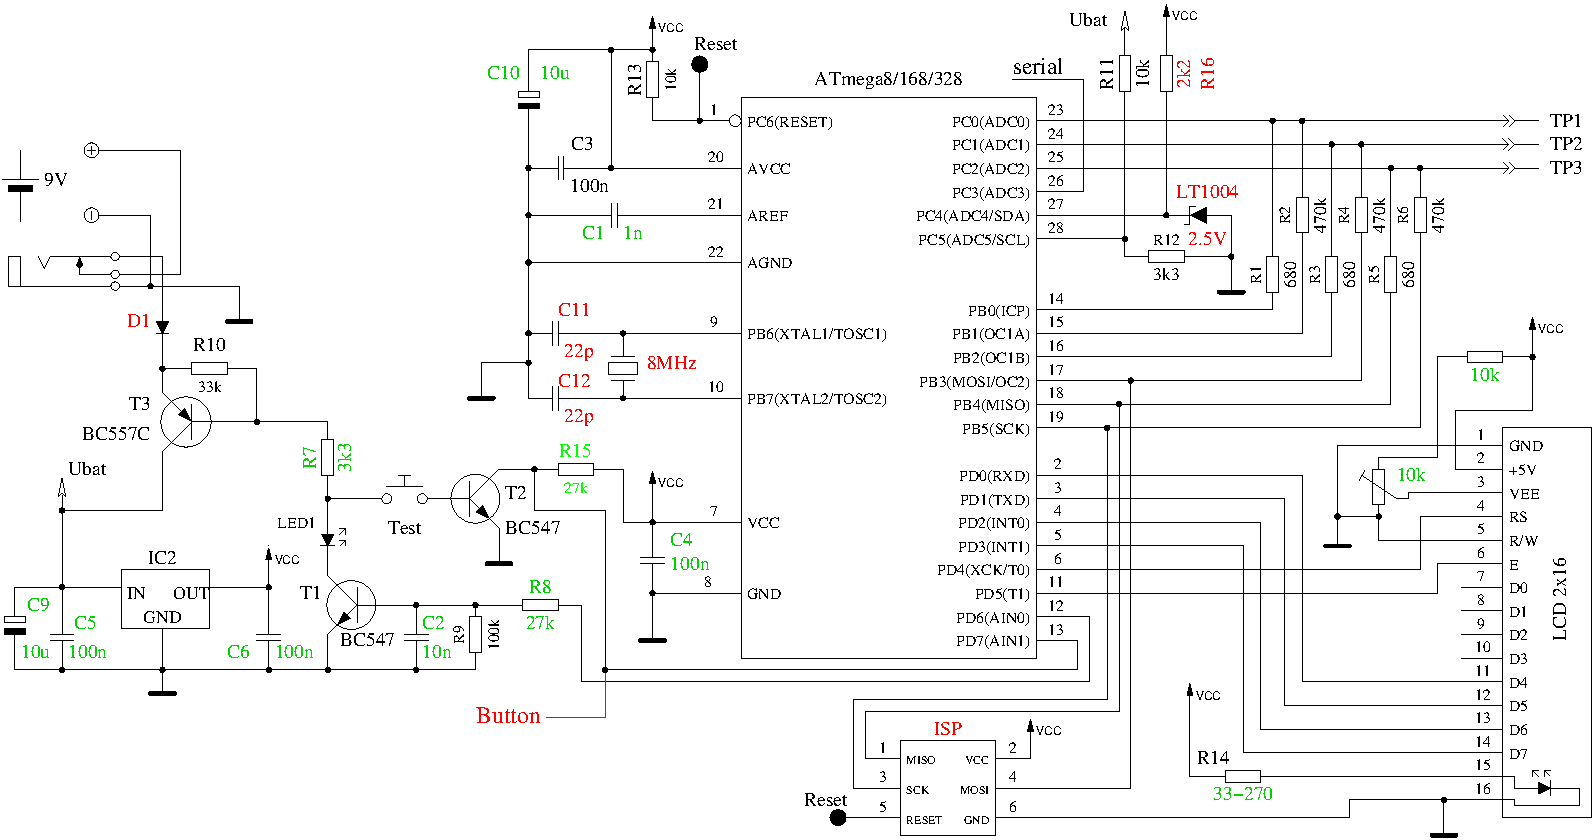
\includegraphics[width=1.\textwidth]{../FIG/ttester.pdf}
\caption{Nové schéma universálního testeru}
\label{fig:ttester}
\end{figure}

Tabulka~\ref{tab:displayCon} zobrazuje přiřazení PD portů různých verzí displejů
a přiřazení dalších funkcí.
Ve všech variantách této tabulky by měly být možné další přídavné funkce .
Signál LCD-CE je k disposici v rozhraní SPI na portu ATmega.  Vstupní CE (Chip Enable)
Vstup CE (Chip Enable) řídicí jednotky může být také připojen k GND namísto připojení k výstupu LCD-CE.

\begin{table}[H] \small
  \begin{center}
    \begin{tabular}{| c || c | c | c | c | c | c |}
    \hline
           & Character     & ST7565 LCD & ST7920 LCD     & NT7108 LCD  & SSD1306     & Přídavné funkce \\
      Port & LCD           &   SPI      & serial         & serial      &   I\textsuperscript{2}C      & \\
    \hline
    \hline
    PD0    &  LCD-D4       &  LCD-REST  & LCD-REST       & 595-PCLK        &            & \\
    \hline
    PD1    &  LCD-D5       &  LCD-RS    &                & LCD-CS2     &             & Rotační koder-2 \\
    \hline
    PD2    &  LCD-D6       &  LCD-SCLK  & LCD-B0         & 164-595-CLK &  LCD-SDA    & \\
    \hline
    PD3    &  LCD-D7       &  LCD-SI    &                & LCD-CS1     &             & Rotační koder-1 \\
    \hline
    PD4    &  LCD-RS       &            &                & LCD-RS      &             & Frekvenční čítač \\
           &               &            &                & 164-595-SER &             &                \\
    \hline
    PD5    &  LCD-E        &  (LCD-CE)  & LCD-EN         & LCD-EN      &   LCD--SCL  & \\
    \hline
    PD7    & Tlačítko & Tlačítko & Tlačítko & Tlačítko & Tlačítko & \\
    \hline
    \end{tabular}
  \end{center}
  \caption{Přiřazení kontaktů pro různé displeje}
  \label{tab:displayCon}
\end{table}

Aby bylo dosaženo jednoduššího propojení displeje s ATmega na DPS, je možné softwarově přiřadit portu D jiné funkce. Následující tabulka 2.2 zobrazuje změny přiřazení pinů pro textové displeje a alternativní připojení grafických displejů pomocí mikrokontroléru ATmega328. Kromě toho je zobrazeno přiřazení Portových vstupů pro přídavné funkce.
Pokud používáte grafický displej s možností mřížky(STRIP\_GRID\_BOARD=1)
není funkce čítače frekvence možná, protože displej používá port PD4 (T0).
Přesto se o toto přiřazení jedna čínská verze s grafickým zobrazením pokouší.
Ve většině případů jsou verze desek, které jsou vybaveny textovým displejem, pro dodatečné vybavení
funkce čítače frekvence a ovládání s rotačním kodérem, vhodnější, protože jsou požadováné
signály na pinech displeje k dispozici . 


\begin{table}[H]
  \begin{center}
    \begin{tabular}{| c || c | c | c | c |}
    \hline
           & Char. LCD      & ST7565 LCD     & ST7565 LCD   & Přídavné funkce \\
      Port &    =1          &    =1          &    =5        &  \\
    \hline
    \hline
    PD0    &  Tastensignal  &                &              &  \\
    \hline
    PD1    &  LCD-D7        & LCD-SI         &  LCD-A0 (RS) &  Rotační koder-2 \\
    \hline
    PD2    &  LCD-D6        & LCD-SCLK       &  LCD-REST    &  \\
    \hline
    PD3    &  LCD-D5        & LCD-A0 (RS)    &  LCD-SCLK    &  Rotační koder-1 \\
    \hline
    PD4    &  LCD-D4        & LCD-REST       &  LCD-SI      &  Frekvenční čítač \\
    \hline
    PD5    &  LCD-E         & (LCD-CE)       &              &  \\
    \hline
    PD7    & LCD-RS         & Tlačítko   & Tlačítko &  \\
    \hline
    \end{tabular}
  \end{center}
  \caption{Alternativní přiřazení pinů s možností STRIP\_GRID\_BOARD}
  \label{tab:grid-change}
\end{table}

\section{Přídavné funkce pro universální tester}
\subsection{Ochrana ATmega vstupů}  

Pro lepší ochranu ATmega vstupů může být tester rozšířen o relé nebo  diody
podle schématu zapojení~\ref{fig:relay_addon} .
Bez napětí spojené rozpínací kontakty relé chrání ATmega už při vypnutí.
Tyto kontakty budou softwarem rozpojeny pouze v době měření.
Instalace přepěťové ochrany s diodami také zvyšuje šance ATmega přežít připojení
kondenzátoru s vyšším zbytkovým napětím.
Úplná ochrana ale není možná. Proto by měly být před měřením vždy kondenzátory vybité.
\begin{figure}[H]
 \begin{subfigure}[b]{.5\textwidth}
  \centering
  \begin{overpic}[width=.78\textwidth]{../FIG/relay_addon.pdf}
  \color{black}
  \put(78,36){\makebox(0,0)[lb]{\footnotesize {VCC nebo Ubat}}}  
  \put(78,32){\makebox(0,0)[lb]{\footnotesize {závisle na U}\scriptsize {relé}}}
  \end{overpic}
  \caption{s relé}
 \end{subfigure}
 \begin{subfigure}[b]{.5\textwidth}
  \centering
  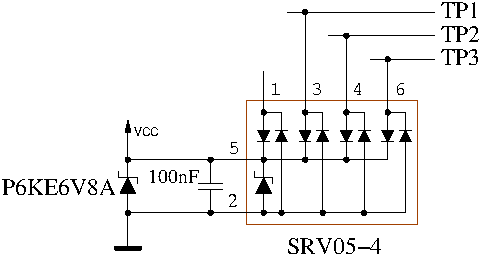
\includegraphics[width=.78\textwidth]{../FIG/diode_addon.pdf}
  \caption{S diodami}
 \end{subfigure}
 \caption{Dodatečná ochrana ATmega vstupů}
 \label{fig:relay_addon}
\end{figure}
Ještě lepší ochranu nabízí relé vybavené s 3mi přepínacími kontakty jak je znázorněno
na obrázku~\ref{fig:relay_um_addon} .
Výstupní proud je zde omezen odpory a vstupy ATmega jsou v chráněném stavu odděleny.
Nesmíme zapomínat, že testovací přístroj zůstává přesto, během měření, nechráněný.

\begin{figure}[H]
\centering
 \begin{overpic}[width=.58\textwidth]{../FIG/relay_um_addon.pdf}
  \color{black}
 \put(78,42){\makebox(0,0)[lb]{\footnotesize {VCC nebo Ubat}}}  
	 \put(78,38){\makebox(0,0)[lb]{\footnotesize {závisle na U}\scriptsize {relé}}}  
 \end{overpic}
\caption{Vylepšená ochrana s relé}
\label{fig:relay_um_addon}
\end{figure}
\subsection{Měření Zenerova napětí}

Není-li výstup sériových textů potřebný, může být  pin PC3 ATmega použít pro měření externího napětí.
Napětí lze nastavit volitelným přepínačem odporu 10:1 až do \(50V\) a lze ho použit
také k měření Zenerova napětí diody.
Proudově omezený zdroj napájení s výstupním napětím až k \(50V\) může být
připojen k \(0V\)-signálu pinů ATmega PD7, k zjištění Zenerova napětí diody.
Návrh na toto rozšíření je zobrazen na obrázku~\ref{fig:zener}.
Pokud je tlačítko stisknuto zobrazuje tester externí napětí.
Pokud je tlačítko stisknuto stoupá spotřeba baterie asi na \(40mA\) .

\begin{figure}[H]
\centering
  \begin{overpic}[width=.90\textwidth]{../FIG/zener_exp.pdf}
  \color{black}
   % \put(42,25.5){\makebox(0,0)[cb]{tlačítko}} 
  \put(5,20){\makebox(0,0)[rb]{\textcolor{red}{externí}}}  
  \put(5,17){\makebox(0,0)[rb]{\textcolor{red}{napětí}}}  
  \put(33,24){\makebox(0,0)[rb]{Má místo na desce!}} 
  \put(42,6){\makebox(0,0)[lb]{Musí být externě umístěno!}}    
  \end{overpic}
\caption{Rozšíření o měření Zenerova napětí}
\label{fig:zener}
\end{figure}
Dělič napětí 10:1 lze s ATmega328 použít i bez měniče napětí.
Bez stisknutého tlačítka měnič napětí není v provozu,
čímž je možné měřit externí napětí (např. Napětí baterie) na portu pro měření Zenerových diod.
Lze měřit pouze kladná stejnosměrná napětí až do \(50V\) .
Takže musíte věnovat pozornost správné polaritě.

\subsection{Frekvenční generátor}

Pomocí sekce menu ATmega lze také přidat frekvenční generátor
s frekvencí od \(1Hz\) do \(2MHz\) .
Výstupní \(5V\) signál je vyveden přes \(680\Omega\)-odpor na TP2.
Jako zem lze použít nulovou svorku na přídavném zařízení pro test zenerových diod nebo
pin TP1 testeru.
TP3 je také připojen na kostru přes \(680\Omega\) odpor.
Samozřejmě, lze ATmega port PB2 použít také jako obvod pro zesilování externího výstupního signálu.
V tomto případě by měl vstup tohoto okruhu nepředstavovat žádnou kapacitní zátěž pro ATmega výstup.

\subsection{Frekvenční čítač}
\label{sec:frequency_counter}

Pro tuto volbu čtení kmitočtu je nutné malé rozšíření.
Vstup pro měření kmitočtu je použit pin PD4 (T0 / PCINT20) ATmega. Tento pin je zároveň použitý
pro LCD připojení.
V normálním uspořádání se jedná o LCD-RS, při displejem s rozvržením mřížky je to LCD-D4.
Pro oba signály je pin PD4 přepnout na vstup a použít pro měření,
pokud není potřeba zobrazení na LCD displeji.
LCD displej se zajímá  o tento signál pouze při přepnutí LCD-E na GND.
Pro zavedení zkušebního signálu je nutný alespoň sériový odpor \(270\Omega\).
Lepší je použít schéma podle obrázku~\ref{fig:FreqMes}.
Napětí na kontaktu PD4 (LCD-RS nebo LCD-D4) by měla být nastavena na hodnotu asi \(2,4V\),
bez připojeného ATmega nebo režimu měření frekvence,
aby byla dosažena nejvyšší citlivost pro vstupní signál.
Displej by ale měl být zapojený,protože jeho ,,Pull-Up'' odpory mění napětí.

\begin{figure}[H]
\centering
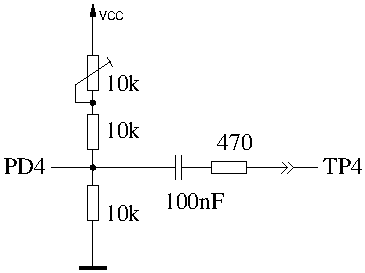
\includegraphics[width=.4\textwidth]{../FIG/Frequency_addon.pdf}
\
\caption{Rozšíření pro měření frekvence}
\label{fig:FreqMes}
\end{figure}
 
\subsection{Rotační pulzní enkodér}
 
\begin{wrapfigure}{r}{0.4\textwidth}
\vspace{-1.5\baselineskip}
\begin{center}
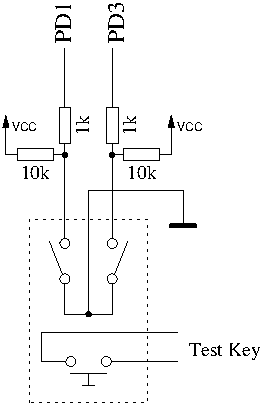
\includegraphics[width=0.30\textwidth]{../FIG/rotary_extension.pdf}
 % \put(47,6){\makebox(0,0)[lb]{tlačítko}}    
\end{center}
\vspace{-0.5\baselineskip}
\caption{Rozšíření o rotační pulzní snímač}
\vspace{-0.5\baselineskip}
\label{fig:RotExt}
\end{wrapfigure}


Pro snadnější ovládání funkce menu pro ATmega328 může být obvod rozšířen o rotační snímač
s tlačítkem.
Schéma~\ref{fig:RotExt} udává výchozí přiřazení pro běžný LCD displej.
Všechny vývody pro snímač impulzů jsou k dispozici na konektoru LCD displeje. 
Rotační enkodér lze proto většinou snadno doplnit.
V mnoha případech je grafický displej spojen s deskou s adaptérem na napájecí liště LCD.
To je důvod, proč dodatečné vybavení pulzního snímače není ani v tomto případě obtížné.
Obrázek~\ref{fig:RotEnc} zobrazuje dvě verze snímačů.
První verze má dvakrát tolik krokových poloh (detent) pro otáčku než impulsů pro otáčku.
Druhá verze má stejný počet impulzů na otáčku jako krokových poloh.
Některé snímače mají spínací hranu jednoho ze dvou spínačů přesně v zarážkové poloze.

\begin{figure}[H]
\centering
 \begin{overpic}[width=.87\textwidth]{../FIG/rotary_encoder.pdf}
  \color{black}
  \put(90,71.5){\makebox(0,0)[lb]{kontakt A}}
  \put(90,62){\makebox(0,0)[lb]{kontakt B}}
  \put(90,29){\makebox(0,0)[lb]{kontakt A}}
  \put(90,19){\makebox(0,0)[lb]{kontakt B}}
	 \put(6,6){\makebox(0,0)[rb]{\footnotesize {krok:}}}
	 \put(6,48.5){\makebox(0,0)[rb]{\footnotesize {krok:}}}
	 \multiput(23.5,53)(24.6,0){3}{\footnotesize {zarážka}}
	 \multiput(11,10)(12.3,0){6}{\footnotesize {zarážka}}
  \put(52,43){\makebox(0,0)[cb]{\large {Verze 2}}}
  \put(52,1){\makebox(0,0)[cb]{\large {Verze 1}}}
 \end{overpic}
\caption{Dvě různé verze snímačů impulzu}
\label{fig:RotEnc}
\end{figure}
 
Obrázek~\ref{fig:RotBounce} zobrazuje pulzní snímač, který nejenže
má kontakty které po pohybu kmitají,\\ ale u kterého jeden z nich stojí
v aretovaném stavu (detent) v nejisté poloze.\\ Program monitoruje každou změnu stavu spínače
a uloží ji v cyklické vyrovnávací paměti.\\ Jakmile dojde ke změně stavu jsou i dva předchozí
stavy známé a zkontrolovány.
Celkově mohou být pro jeden cyklus spínacích stavů použity čtyři stavové sekvence pro každý směr otáčení
nastavitelné.\\Má-li kodér pro jeden cyklus pouze jednu zarážku, stačí dotaz
jednoho páru těchto stavových sekvencí pro počítání zarážek v obou směrech (WITH\_ROTARY\_SWITCH=2 nebo 3).\\
U kodéru s dvěma zarážkami pro cyklus, jak je znázorněno na obrázku~\ref{fig:RotBounce} ,
musí být dotazovány dva páry (WITH\_ROTARY\_SWITCH=1).
U impulsních snímačů bez zarážek lze nastavit parametr WITH\_ROTARY\_SWITCH podle potřeby na
2 nebo 3 pro nejnižší citlivost, na 1 pro střední citlivost a na 5 pro nejvyšší citlivost.
Tímto způsobem dotazu se lze vyhnout výkyvu nastavení(počítadlo nahoru a dolů) ale umožní že
bude v nevýhodné pozici spínací polohy, v aretovaném stavu, jeden impuls vynechán.
\begin{figure}[H]
\centering
  \begin{overpic}[width=.87\textwidth]{../FIG/rotary_bouncing.pdf}
  \color{black}
  \put(90,39){\makebox(0,0)[lb]{kontakt A}}
  \put(90,30){\makebox(0,0)[lb]{kontakt B}}
  \multiput(11,23)(28,0){3}{\footnotesize {zarážka}}
  \put(7,20){\makebox(0,0)[rb]{krok:}}
  \put(5,12){\makebox(0,0)[lb]{Možné polohy z zleva do prava:}}      
  \end{overpic}
  \caption{Impulzní snímač s kmitavými kontakty}
  \label{fig:RotBounce}
\end{figure}
Pokud není impulsní otoční spínač dostupný nebo požadován, je možné, pro obsluhu funkci nahoru a dolů,
použít také dvě tlačítka.
V tomto případě musí být volba WITH\_ROTARY\_SWITCH nastavena na 4, aby mohl program
patřičně reagovat.

\subsection{Připojení grafického displeje}

Díky práci Wolfganga Sch. za podporu čínské verze s grafickým LCD displejem o rozměrech 128x64 pixelů
lze nyní také připojit grafický LCD displej s řídící jednotkou ST7565.
Protože je řídicí jednotka ST7565 řízena sériově, jsou zapotřebí pouze čtyři signály.
Tím se uvolní dva piny portu D pro jiné použití.
Procesor ATmega by měl mít nejméně 32k flash paměti.
Řídicí jednotka ST7565 pracuje s provozním napětím \(3,3V\) .
Proto je nutný přídavný regulátor s tímto napětím.
Podle datového listu řídicího systému se k jeho vstupům nemohou přímo připojit žádné \(5V\) signály.
Proto je v rozšíření na obrázku \ref{fig:ST7565lcd} další CMOS 74HC4050
určený pro nastavení úrovně.\
Můžete také zkusit nahradit 74HC4050 čtyřmi odpory přibližně \(2,7k\Omega\) .
Pokles napětí na odporech zabraňuje tomu, aby se to  \(3,3V\)-napětí nedostalo přes ochranné diody
ATmega vchodů a ty \(5V\) ATmega-výstupy nestoupli přes tu \(3,3V\)-hranici.
Jest-li je tento tvar signálu ST7565 řadičem přijat, musíte vyzkoušet. 74HC4050 je v každém
případě lepší řešení.
 
\begin{figure}[H]
\centering
 \begin{overpic}[width=.814\textwidth]{../FIG/ST7565lcd.pdf}
  \color{black}
  \put(88,10){\makebox(0,0)[lb]{zadní světlo}}  
  \put(88,7){\makebox(0,0)[lb]{LED}}   
 \end{overpic}
\caption{Připojení grafického displeje s ovladačem  ST7565}
\label{fig:ST7565lcd}
\end{figure}

Tabulka \ref{tab:spi-processor} zobrazuje další možnosti připojení
pro ATmega328 a další procesory s SPI (LCD\_INTERFACE\_MODE=4)
nebo 3LINE (LCD \_INTERFACE \_MODE = 3)  rozhraním. Různé zadání pro
procesor je s volbou STRIP\_GRID\_BOARD možné.
Přiřazení jsou definována v souboru config.h. 
Pokud je vyžadováno více variant obsazenosti, měly by tyto být
určeny dalšími kódovými čísly možností v STRIP \_GRID\_BOARD
a pak přidány do config.h.

\begin{table}[H]
  \begin{center}
    \begin{tabular}{| c || c | c | c | c | c | c | c |}
    \hline
 Procesor  & m644  & m1280 & m1280  & m328 & m328 & m328 & m328 \\
STRIP\_GRID\_BOARD &       &   -   &   1    &  -   &  1   &  2   &  5   \\
    \hline
    \hline
Signal:     &       &       &        &      &      &      &      \\
  RES       &  PB4  & PA0   &  PA4   & PD0  & PD4  & PD0  & PD2 \\
    \hline
  EN, CLK   &  PB6  & PA2   &  PA2   & PD2  & PD2  & PD2  & PD3 \\
    \hline
  RS, D/C   &  PB5  & PA1   &  PA3   & PD1  & PD3  & PD3  & PD1 \\
    \hline
  B0, MOSI  &  PB7  & PA3   &  PA1   & PD3  & PD1  & PD1  & PD4 \\
    \hline
  CE, CS    &  PB3  & PA4   &  PA5   & PD5  & PD5  & PD5  & PD5 \\
    \hline
    \end{tabular}
  \end{center}
  \caption{Přiřazení SPI pinů SPI pro různé procesory}
  \label{tab:spi-processor}
\end{table}

Normálně je řídicí jednotka ST7565 nebo SSD1306 připojena k rozhraní 4-Wire SPI.
Řídicí jednotka SSD1306 může také používat I\textsuperscript{2}C- rozhraní s PD2 jako SDA- a PD5 jako SCL-signál.
SDA- a SCL-signály musí mít ,,Pull-up'' odpor s hodnotou asi \(4,7k\Omega\) k \(3,3V\) .
Možnost připojení je zobrazena na obrázku \ref{fig:ssd1306i2c}.
Před použitím ,,Pull-up'' odporů na \(5V\) je nutné zkontrolovat, zda vstupy toto napětí tolerují.
Obvykle jsou vstupy regulátoru diodami na \(3.3V\) chráněny.
ATmega výstupy ATmega jsou při použití I\textsuperscript{2}C-rozhraní jen na  \(0V\) přepnuty.
Před připojením displeje je však třeba zajistit, že byl načten do ATmega program
pro I\textsuperscript{2}C rozhraní.
Pokud byl program načten pro jiné rozhraní, jsou ATmega výstupy přepnuty na \(5V\) .
Vzhledem k tomu, že jsem zjistil vliv na výsledky testů při připojení OLED modulů přes VCC kontakt,
doporučuji pro oddělení přidat sériový odpor s \(68\Omega\) a další \(10\mu F\) blokovací kondenzátor. 
Namísto \(68\Omega\) odporu lze použít tlumivku s asi \(1mH\) .
Bez tohoto opatření byly na mém testeru zobrazeny zbytkové proudy kolektorů v bipolárních tranzistorech s OLED.
Kromě toho je třeba zkontrolovat přiřazení pinů na modulu OLED, některé moduly mají GND a VCC obráceně!

\begin{figure}[H]
\centering
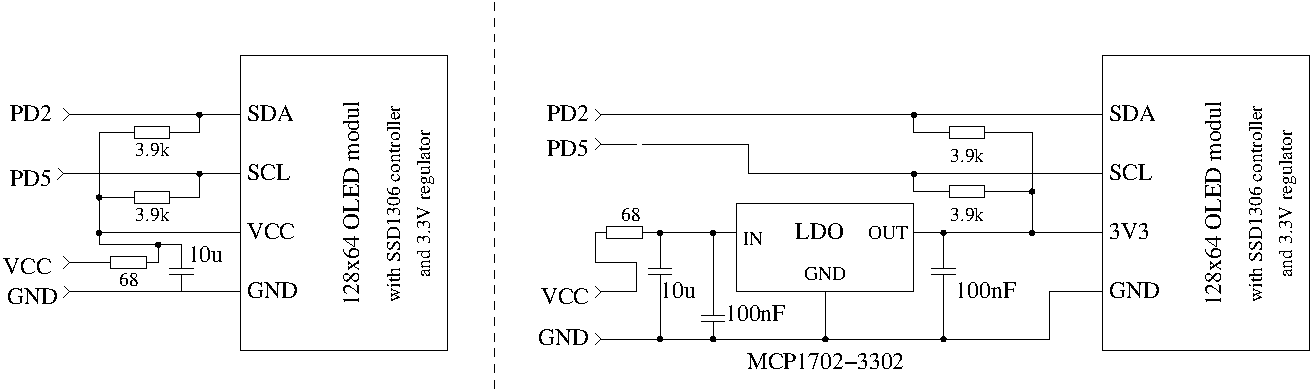
\includegraphics[width=.814\textwidth]{../FIG/SSD1306_I2C.pdf}
\caption{Připojení grafického OLED displeje s I\textsuperscript{2}C rozhraním}
\label{fig:ssd1306i2c}
\end{figure}

U procesorů řady ATmega644 jsou pro připojení použité piny PD3 (SCL) a PD4 (SDA) místo PD5 a PD2.
Řada procesorů ATmega1280 používá piny PA5 (SCL) a PA4 (SDA).
Výměna textového displeje za grafický je s adaptérovou deskou možná.
Na LCD konektoru jsou všechny potřebné datové a napájecí signály k dispozici.
O něco jednodušší je připojení grafického displeje s řadičem ST7920, protože
regulátor běží na provozním napětí \(5V\) .
Displej by měl mít 128x64 viditelných pixelů.
Zobrazovací modul s řídicí jednotkou ST7920  lze připojit jako 4 bitové paralelní rozhraní nebo
pomocí speciálního sériového rozhraní jak ukazuje obrázek \ref{fig:ST7920lcd} .

\begin{figure}[H]
\centering
 \begin{overpic}[width=.698\textwidth]{../FIG/ST7920interface.pdf}
  \color{black}
  \put(20,1){\makebox(0,0)[cb]{sériový modus}}  
  \put(80,1){\makebox(0,0)[cb]{4-bitový paralelní modus}}   
 \end{overpic}
\caption{Připojení displeje pomocí ovladače ST7920}
\label{fig:ST7920lcd}
\end{figure}

Pro oba typy připojení musí být software speciálně nakonfigurován.
Makefile volba ,,WITH\_LCD\_ST7565 = 7920'' musí být v každém případě nastavena.
Pro sériový Typ připojení musí být také volba "CFLAGS + = -DLCD \_INTERFACE \_MODE=5" zvolená.
Tabulka~\ref{tab:ser-processor} ukazuje přiřazení signálů sériového portu
připojení typu 5 (ST7920) a 7 (SSD1803) pro různé procesory.

\begin{table}[H]
  \begin{center}
    \begin{tabular}{| c || c | c | c | c |}
    \hline
 Processor  & m644  & m644 & m1280  & m328 \\
STRIP\_GRID\_BOARD &       &   1   &        &     \\
    \hline
    \hline
Signal:     &       &       &        &         \\
  EN        &  PB3  & PB6   &  PA5   & PD5     \\
    \hline
  B0, R/W   &  PB4  & PB7   &  PA4   & PD2      \\
    \hline
  RESET     &  PB2  & PB4   &  PA0   & PD0      \\
    \hline
    \end{tabular}
  \end{center}
  \caption{Zapojení Sériového portu pro různé procesory}
  \label{tab:ser-processor}
\end{table}

Orientaci displeje může být, stejně jako u všech grafických displejů, nastavena
možností LCD\_ST7565\-\_H\_FLIP a LCD\_ST7565\-\_V\_FLIP.
Zvláštním případem jsou displeje s řadiči NT7108 nebo KS0108 (S6B0108). Jelikož jsou ovládané
pouze s 8bitovým paralelním rozhraním. U nich je třeba použít externí sériově paralelní převodník.
Nejjednodušší řešení se mi zdá použít čip 74HCT164 nebo 74HCT595.
Odpovídající návrh schematu je zobrazen na obrázku \ref{fig:NT7108lcd} .

\begin{figure}[H]
  \begin{subfigure}[b]{.5\textwidth}
    \centering
    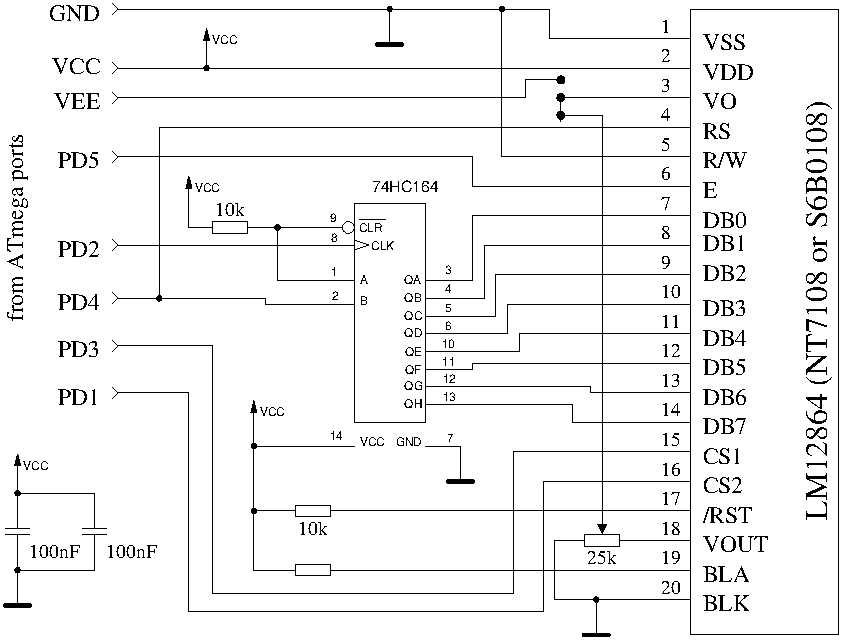
\includegraphics[width=.9\textwidth]{../FIG/ST7108serial164.pdf}
    \caption{s 74HCT164}
  \end{subfigure}
  \begin{subfigure}[b]{.5\textwidth}
    \centering
    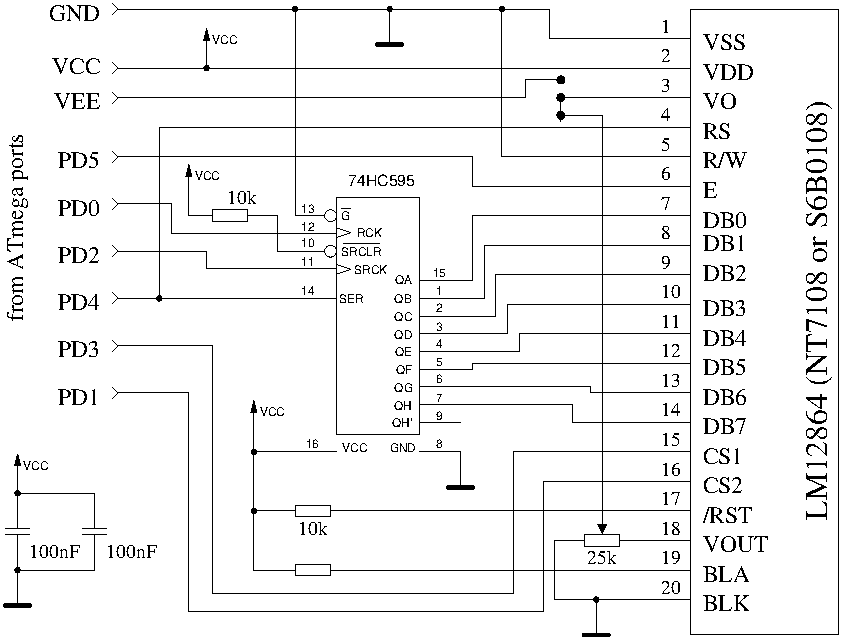
\includegraphics[width=.9\textwidth]{../FIG/ST7108serial595.pdf}
    \caption{s 74HCT595}
  \end{subfigure}
  \caption{Připojení grafického displeje s ovladačem NT7108}
  \label{fig:NT7108lcd}
\end{figure}

Je třeba zkontrolovat pořadí pinů na vašem LCD displeji, některé moduly mají jinou sekvenci signálů.
Několik různých přiřazení pinů z datových listů řady ABG128064 zobrazuje tabulka~\ref{tab:NT7108types}.

\begin{table}[H]
  \begin{center}
    \begin{tabular}{| c || c | c | c | c |}
    \hline
           & 128064H  &  128064G  & 128064C  & 128064B \\
    Signal &         &          &         &         \\
    \hline
    \hline
  VDD (5V) &   1     &  2       &   4     & 2       \\
    \hline
  VSS (GND) &   2     &  1       &   3     & 1       \\
    \hline
 VO (Drive) &   3     &  3       &  (5)    & 3       \\
    \hline
  DB0-DB3   &   4-7   &  7-10    &   9-12  & 7-10    \\
    \hline
  DB4-DB7   &   8-11  &  11-14   &   13-16 & 11-14   \\
    \hline
  CS1       &   12    &  15      &   1     & 15      \\
  CS2       &   13    &  16      &   2     & 16      \\
    \hline
  Reset     &   14    &  17      &   -     & 17      \\
    \hline
  R/W       &   15    &  5       &   7     & 5       \\
    \hline
  RS        &   16    &  4       &   6     & 4       \\
    \hline
  E         &   17    &  6       &   8     & 6       \\
    \hline
  VEE       &   18    &  18      &   -     & 18      \\
    \hline
  LEDA      &   19    &  19      &   17    & (19)      \\
  LEDK      &   20    &  20      &   18    & -      \\
    \hline
    \end{tabular}
  \end{center}
  \caption{Přiřazení pinů různých NT7108 modulů}
  \label{tab:NT7108types}
\end{table}

\begin{table}[H]
  \begin{center}
    \begin{tabular}{| c || c | c | c |}
    \hline
 Procesor  & m644  &  m1280  & m328 \\
    \hline
    \hline
  EN        &  PB3  &  PA5   & PD5     \\
    \hline
  RS        &  PB2  &  PA4   & PD4      \\
  B0        &  PB2  &  PA4   & PD4      \\
    \hline
  CS1       &  PB7  &  PA3   & PD3      \\
    \hline
  CS2       &  PB5  &  PA1   & PD1      \\
    \hline
  CLK       &  PB6  &  PA2   & PD2      \\
    \hline
  PCLK      &  PB4  &  PA0   & PD0      \\
    \hline
    \end{tabular}
  \end{center}
  \caption{Zapojení sériového portu NT7108 pro různé procesory}
  \label{tab:7108-processor}
\end{table}

Je také možné použít displeje s řadičem PCF8814, jako jsou např
jsou nainstalovány v telefonu Nokia 1100. Přitom je nutné zjistit, jaké rozhraní modulu displeje
používá. Řadič PCF8814 podporuje rozhraní SPI jako 3-řádkové a 4-řádkové,
rozhraní, I\textsuperscript{2}C-rozhraní a speciální 3-řádkové rozhraní u kterého se
Datový / instrukční signál přenáší jako první sériový bit.
Displej má pouze 96x65 pixelů, takže žádné velké grafické symboly pro
Tranzistory nelze s tímto regulátorem použít. Zobrazení je tedy podobné jako u textového displeje.
Stejně jako u většiny grafických displejů je provozní napětí \(3,3V\) .
Proto je úprava signálu na \(5V\) ATmega výstupy nutná.
Pro SPI a 3 řádkové rozhraní je možné ATmega výstupy pomocí volby LCD\_SPI\_OPEN\_COL jako
 ,,Open Collector'' výstupy použít.
Vyžadují se však ,,Pull-Up'' odpory nebo se nesmí volba PULLUP\_DISABLE v Makefile použít.
V současné době je vyzkoušeno pouze 3-řádkové rozhraní.
\begin{table}[H]
  \begin{center}
    \begin{tabular}{| c || c | c | c | c |}
    \hline
           &  PCF8814    & PCF8814        & PCF8814     & Přídavné funkce \\
      Port &    SPI      & 3-line         &   I\textsuperscript{2}C      & \\
    \hline
    \hline
    PD0    &   LCD-REST  & LCD-REST       &            & \\
    \hline
    PD1    &   LCD-D/C   & LCD-SCE        &             & rotační snímač-2 \\
    \hline
    PD2    &   LCD-SCLK  & LCD-SCLK       &  LCD-SDIN   & \\
    \hline
    PD3    &   LCD-SDIN  & LCD-SDIN       &             & rotační snímač-1 \\
    \hline
    PD4    &             &                &             & měřič frekvence \\
    \hline
    PD5    &             & LCD-EN         &   LCD-SCLK  & \\
    \hline
    \end{tabular}
  \end{center}
  \caption{Přiřazení pinů pro různé varianty připojení řadiče PCF8814}
  \label{tab:PCF8814-con}
\end{table}

K dispozici je také podpora pro řadič PCF8812 s rozlišením 102x65 pixelů,
ale zcela netestován.

\subsection{Připojení grafického barevného displeje}

Čínští prodejci nabízejí levné barevné moduly s SPI rozhraním.
Na obrázku \ref{fig:Color_both} je zadní část dvou podporovaných modulů 128x128 pixelů
a 128x160 pixelů.
Tyto moduly jsou velmi malé, takže i texty a symboly jsou velmi malé.
Ale vzhled je ostrý a jasný.

\begin{figure}[H]
\centering
\includegraphics[width=.46\textwidth]{../PNG/Color_ILI9163_ST7735.jpg}
\caption{zadní strana obou barevných LCD}
\label{fig:Color_both}
\end{figure}

Modul 128x128 pixel používá ILI9163 kontrolér.
Modul 128x160 pixel používá velmi podobný řadič ST7735.
Testoval jsem moduly s adaptérovou deskou, která připojuje
SPI signály  a napájení svorkovnice s normálním textovým displejem.
Přizpůsobení těch \(5V\) ATmega signálů na \(3.3V\) vstupy regulátoru
jsem realizoval sériovými \(10k\Omega\) odpory.
Podsvícení (LED) je pro tyto moduly nezbytné, jinak není znázornění rozpoznatelné. 
Vzhledem k vysokému počtu pixelů ve svislém směru lze na displejích zobrazit více řádků textu.
Na displeji s 128x128 pixelů lze zobrazit až 8 řádků textu s fontem 12x8,
U displeje 128x160 pixelů je dokonce 10 řádků textu.
Na fotografii \ref{fig:Color_PNP} je výsledek měření germaniového tranzistoru na
displeji s 128x128 pixely.

\begin{figure}[H]
\centering
\includegraphics[width=.46\textwidth]{../PNG/Color_PNP_ILI9163.jpg}
\caption{Měření bipolárního PNP tranzistoru}
\label{fig:Color_PNP}
\end{figure}

V současné době se barevné možnosti displejů nepoužívají. Pouze barva pozadí
a barva popředí může být změněna v souboru lcd\_defines.h nebo v makefile.
Používá se 16 bitový barevný model řadičů, barva popředí s konstantami
LCD\_FG \_COLOR a barvu pozadí lze nastavit pomocí konstanty LCD\_BG \_COLOR.

\section{Rady pro stavbu této zkoušečky}

Pro tento přístroj lze použít libovolný LCD displej s minimálně 2x16 znaky a kompatibilním
ovladačem k HD44780.
Člověk by měl věnovat pozornost požadavkům na napájení podsvícení, některé potřebují 
více elektřiny než ostatní.
Zkoušel jsem OLED displeje, ale tyto částečně ovlivňovaly ATmega měření
a já je nedoporučuji. Také načítání zvláštních znaků pro zobrazování odporů působilo
s OLED potíže.
Odpory R1 až R6 jsou pro měření kritické a tyto \(680\Omega\) a \(470k\Omega\) odpory
by měli mít toleranci \(0,1\%\)), k zajištění plné přesností.
Aby byla možná výměna ATmega mikrokontroléru měla by se použit precisní zásuvka.
Je možné použít mikrokontrolér ATmega8, ATmega168 a ATmega328.
Pokud chcete používat všechny funkce, doporučuje se ATmega328.
Každopádně byste měli nejprve vybavit všechny součásti bez mikrokontroléru.
Jako IC2 je doporučen Moderní regulátor nízkého napětí, jako je MCP1702-5002,
protože vyžaduje jen \(2\mu A\) klidový proud a může také dodávat \(5V\) , 
pokud je vstupní napětí pouze \(5,4V\) .
Bohužel není tento řadič pinově kompatibilní s řadičem 78L05 v TO-92 provedení!
Po namontování všech požadovaných komponentů by měla být nejdříve baterie 
nebo napájecí adaptér připojené. LCD by neměl být připojen a mikrokontrolér ještě
nebít v patici.
Při stisknutém tlačítku start byste měli zkontrolovat provozní napětí mikrokontroléru a LCD displeje.
Provozní napětí by mělo zmizet po uvolnění spouštěcího tlačítka.
Pokud bylo provozní napětí správné polarity a velikosti,
měli byste odstranit napájecí zdroj a zasunout mikrokontrolér správně orientovaný.
Buďte opatrní a ujistěte se zda jsou všechny piny mikrokontroléru v zásuvce.
Pak můžete připojit LCD. Zkontrolujte, zda jsou svorky GND a VCC na LCD správně připojeny k modulu.
Když jste si jisti, že je vše správně připojeno, zapněte znova napájení.
Pokud jste již ATmega programovali, můžete použít tlačítko start.
Stisknutím spouštěcího tlačítka by mělo podsvícení na LCD displeji svítit.
Po uvolnění tlačítka by LED na desce měla slabě svítit.
Poznámka: Zajistěte, že používáte správně přeložený software pro váš procesor.
Mějte na paměti, že software pro jednočipový ATmega8 nelze spustit na ATmega168!

\section{Konverze testovací verze po Markusu F..}
\label{sec:change_markus}

\begin{description}
\item[Sledování napětí]  
Problém se projeví okamžitém vypnutím při pokusu o zapnutí.
V ode mne doporučených nastavení pojistek (makefile) je monitorování napětí u
různých verzí ATmega nastavené na \(4V\)  (brown out level).  To je důvod, proč to může působit
problémy při zapnutí testeru, protože pin PD6 se pokouší ten \(100nF\)-kondenzátor C2 
přímo připojit. To může vést k nežádoucímu poklesu \(5V\)  napětí.
Kondenzátor C2 lze jednoduše snížit na \textless~\(10nF\) . Pokud je to možné, měl by být
místo přímého připojení PD6 ke kondenzátoru použít odpor \textgreater~\(220\Omega\) k připojení.

\item[Zlepšení spouštění chování]
Často se ukazuje chyba, že se přístroj při stisknutí tlačítka zapne, ale při uvolnění tlačítka
zase vypne. Problém se vyskytuje častěji když po-zadní osvětlení displeje LCD vyžaduje hodně energie.
Odpor R7 na bási PNP tranzistoru T3 s \(27k\Omega\)  byl optimalizován na velkou úsporu energie.
Odpor je třeba lépe snížit na \(3,3k\Omega\) aby také při nižším napětí baterie nebo při použití
PNP tranzistoru T3 s nízkým proudovým zesílením bylo jisté zapnutí zajištěno.

\item[Doplňkový pull-up odpor na PD7]
Chyba je signalizována tím, že se na zkoušečce po krátkém čase a zobrazení zprávy
"Časový limit" vypne. Software je ve výchozím nastavení konfigurován s (volbou PULLUP\_DISABLE),
čémž jsou interní Pull-Up-odpory odpojeny.
Výsledkem je, že úroveň na pinu PD7 není definována, pokud není tlačítkem nebo s T2 přepnut na GND potenciál.
Externí  Pull-Up-odpor s \(27k\Omega\) k VCC vylučuje tuto chybu.

\item[Kondenzátor C1 na pinu AREF]
V mnoha provedeních se zde používá kondenzátor s \(100nF\), stejně jako v návrhu Markuse Frejeka.
Při použití ATmega168 / 328, software ale automatický přepíná referenční napětí z  \(5V\) na vnitřní
referenční napětí \(1,1V\) pokud vstupní napětí klesne pod hodnotou \(1V\) .
Tím získáte lepší rozlišení.
Bohužel je přechod z \(5V\) na \(1.1V\) je velmi pomalý, což vyžaduje další čas o \(10ms\) .
Výměna  \(100nF\) kondenzátoru za \(1nF\) sníží výrazně čekací dobu  . Vliv menších kondenzátorů
na kvalitu výsledků měření jsem nezjistil. Dokonce i odstranění kondenzátoru nemá významný vliv.
Ten kdo si přeje tento \(100nF\) kondenzátor nutně zachovat, může v Makefile volbu NO\_AREF\_CAP odstranit,
 a tím čekací dobu v programu aktivovat.

\item[Dovybavení \(8MHz\) krystalu] S trochou dovednosti lze na pájecí straně desky na vchody PB6 Pin9 a PB7 Pin10  \(8MHz\) krystal přímo naletovat. V mé versi jsem si oba \(22pF\) kondenzátory odpustil. U všech zkoušených procesorů, toto řešení fungovalo. Tento dodatek ale není nezbytný.
Taktovací frekvence, ale z důvodu lepší časové konstanty pro měření kondenzátorů v každém případě
hodnotu \(8MHz\). Tuto hodnotu lze také v RC-oscilátorovém provozu nastavit pojistkou.

\item[Odblokování provozního napětí]
V původním schématu zapojení od Markuse F. je pouze jeden blokovací \(100nF\)-kondenzátor
k VCC-napětí (\(5V\)) přítomen. To je příliš málo. Měl by být jak \(100nF\) kondenzátor v bezprostřední
blízkosti ATmega stejně jako \(100nF\) v bezprostřední blízkosti regulátoru napětí. U vchodu do 
řídicí jednotky patří rovněž  \(100nF\) kondenzátor. Další  \(10\mu F\)-elektrolytické (nebo keramické)
kondenzátory na vstupu i výstupu řadiče mohou zvýšit stabilitu napětí.
Keramické \(10\mu F\)kondenzátory typu SMD jsou vhodnější pro dodatečné vybavení a mají
obvykle nižší ESR hodnotu.

\item[Výběr ATmega procesoru]
Základní funkce testovacího přístroje jsou stále s ATmega8 možné.
Přitom je programová paměť téměř na  \(100\%\) využita.
Protože jsou ATmega168 nebo ATmega328 procesory pin kompatibilní s ATmega8,
lze náhradu pouze doporučit. Mezitím  je cena za ATmega328 tak nízká, že ve skutečnosti nic
nehovoří pro ATmega168.
Přístroj s ATmega168 / 328 nabízí následující výhody:
\begin{itemize} \setlength{\itemsep}{-0.4em}
\item Funkce automatického samo-testu s automatickou kalibrací.
\item Zvýšená přesnost automatického přepnutí referenčního napětí ADC.
\item Měření indukčnosti, jejíž hodnota odporu je  \textless~\(2100\Omega\).
\item Měření ESR hodnoty kondenzátorů \textgreater~\(20nF\).
\item Rozlišení měření odporu pod \(10\Omega\) je \(0,01\Omega\).
\item PC3 pin lze použít jako sériový výstup.
\end{itemize}

\item[Chybějící přesná reference]
Normálně by měla být chybějící referenční hodnota rozpoznána při nezapojeném PC4 pinu.
V tomto případě se na druhém řádku při zapnutí neobjeví žádná VCC = x.xV indikace.
Pokud by se přesto tato informace na displeji zobrazila, pomůže\(2,2k\Omega\) odpor na PC4 vchodu.
\end{description}

\section{Pokročilý obvod s ATmega644 nebo ATmega1284}

Pokročilý obvod pro procesory ATmega644 / 1284 byl vyvinut ve spolupráci s Nickem L.
vyvinutým na Ukrajině. Obvod podle obrázku \ref{fig:t644tester} umožňuje test krystalů a rozšířený
frekvenční rozsah pro měření frekvence.
Ačkoli je základní schema velmi podobné obvodu  \ref{fig:ttester} používá jiné přiřazení portů.
Ovládací kodér okruhu \ref{fig:RotExt} může zde být zapojený na PB5 a PB7 (místo na PD1 a PD3). 
Oba signály a také napájecí signály VCC a GND jsou na konektoru ISP k dispozici,
takže zde můžete také připojit modifikace.
16:1-frekvenční dělič 74HC4060 se vždy používá pro vyšší frekvence než \(2MHz\).
Dělič lze také použít pro frekvence od \(25kHz\) do \(400kHz\) pro použití s měřením
doby pro zlepšení rozlišení měřeného kmitočtu.
Pro přepínání provozních stavů (frekvenční dělič a křemenný oscilátor) jsou
použíty analogové spínače 74HC4052.
Tabulka \ref{tab:mega644-display} zobrazuje přiřazení pinů pro mikrokontrolér
ATmega324 / 624/1284 s různými displeji.
To I\textsuperscript{2}C-rozhraní je možné pouze s řadičem SSD1306.
Signály I\textsuperscript{2}C-rozhraní vyžadují ,,Pull-Up''-odpor asi \(4,7k\Omega\) na \(3,3V\).
ATmega výstupy jsou při I\textsuperscript{2}C-rozhraní jen k \(0V\) propojeny.
\begin{table}[H]
  \begin{center}
    \begin{tabular}{| c || c | c | c | c |}
    \hline
      Port & Klasický LCD &  Grafický LCD & Grafický LCD  & Přídavné funkce      \\
           &               &  SPI 4-Wire  &  I\textsuperscript{2}C         &                     \\
    \hline
    \hline
    PB2    &  LCD-RS         &            &             &       \\
    \hline
    PB3    &  LCD-E          & (LCD-CE)   &  LCD-SCL    &       \\
    \hline
    PB4    &  LCD-D4         & LCD-REST   &  LCD-SDA    &       \\
    \hline
    PB5    &  LCD-D5         & LCD-RS     &             & ISP-MOSI \\
           &                 &            &             & kodér 2 \\
    \hline
    PB6    &  LCD-D6         & LCD-SCLK   &             & ISP-MISO \\
    \hline
    PB7    &  LCD-D7         & LCD-SI     &             & ISP-SCK  \\
           &                 &            &             & kodér 1 \\
    \hline
    \end{tabular}
  \end{center}
  \caption{Různé varianty displejových portů}
  \label{tab:mega644-display}
\end{table}

Dokonce i displej s NT7108 (KS0108, S6B0108) ovladačem lze připojit s malou přídavnou deskou DPS na
ATmega644 nebo ATmega1284 připojit tak, jak je znázorněno na obrázku~\ref{fig:NT7108lcd_644}.
Nezapomeňte ale na různé přiřazení pinů modulů zobrazení s řadičem NT7108, jak je uvedeno v
Tabulce~\ref{tab:NT7108types} na straně~\pageref{tab:NT7108types}.

\begin{figure}[H]
  \begin{subfigure}[b]{.5\textwidth}
    \centering
    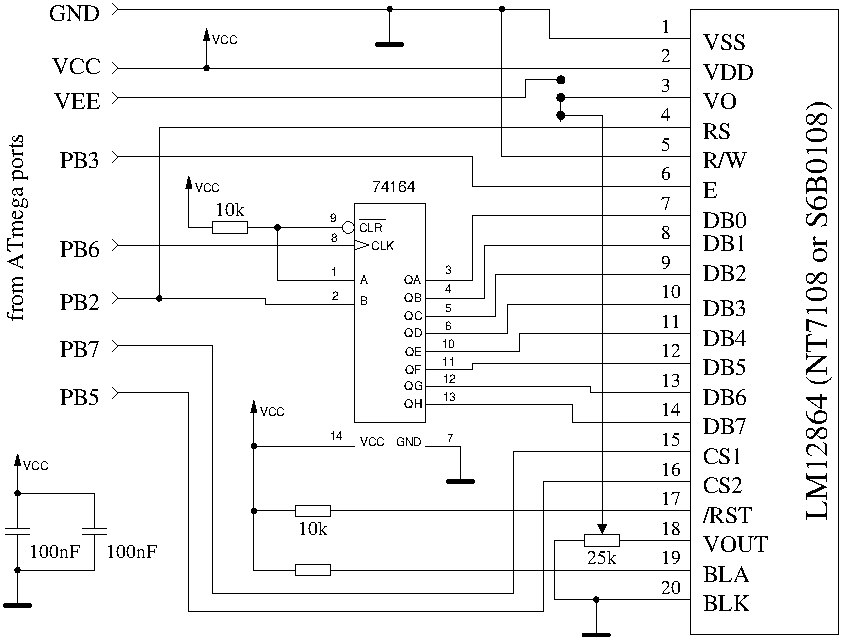
\includegraphics[width=.88\textwidth]{../FIG/ST7108serial164_644.pdf}
    \caption{S 74HCT164}
  \end{subfigure}
  ~
  \begin{subfigure}[b]{.5\textwidth}
    \centering
    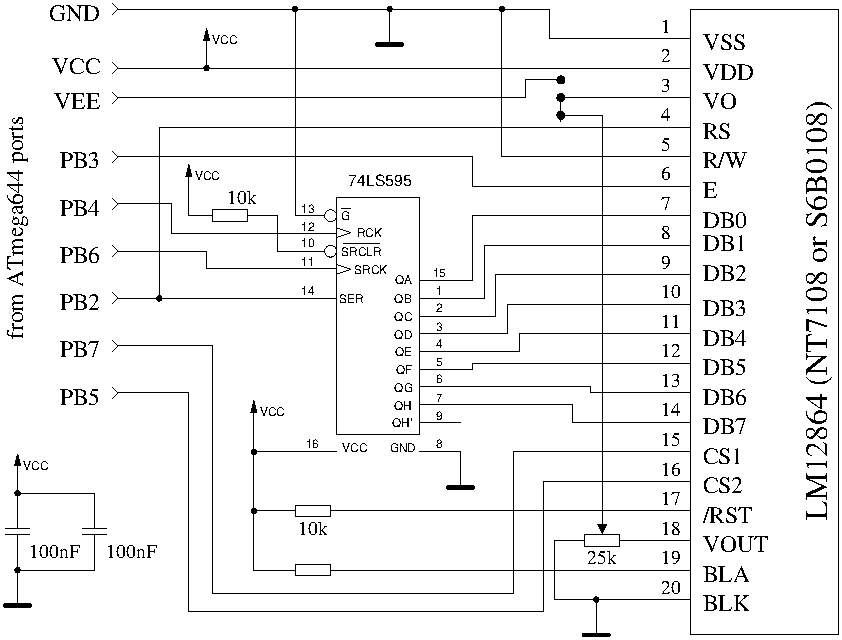
\includegraphics[width=.88\textwidth]{../FIG/ST7108serial595_644.pdf}
    \caption{S 74HCT595}
  \end{subfigure}
  \caption{Zapojení NT7108 ovládače na ATmega644/1284}
  \label{fig:NT7108lcd_644}
\end{figure}


\label{T644}
\begin{figure}[H]
\centering
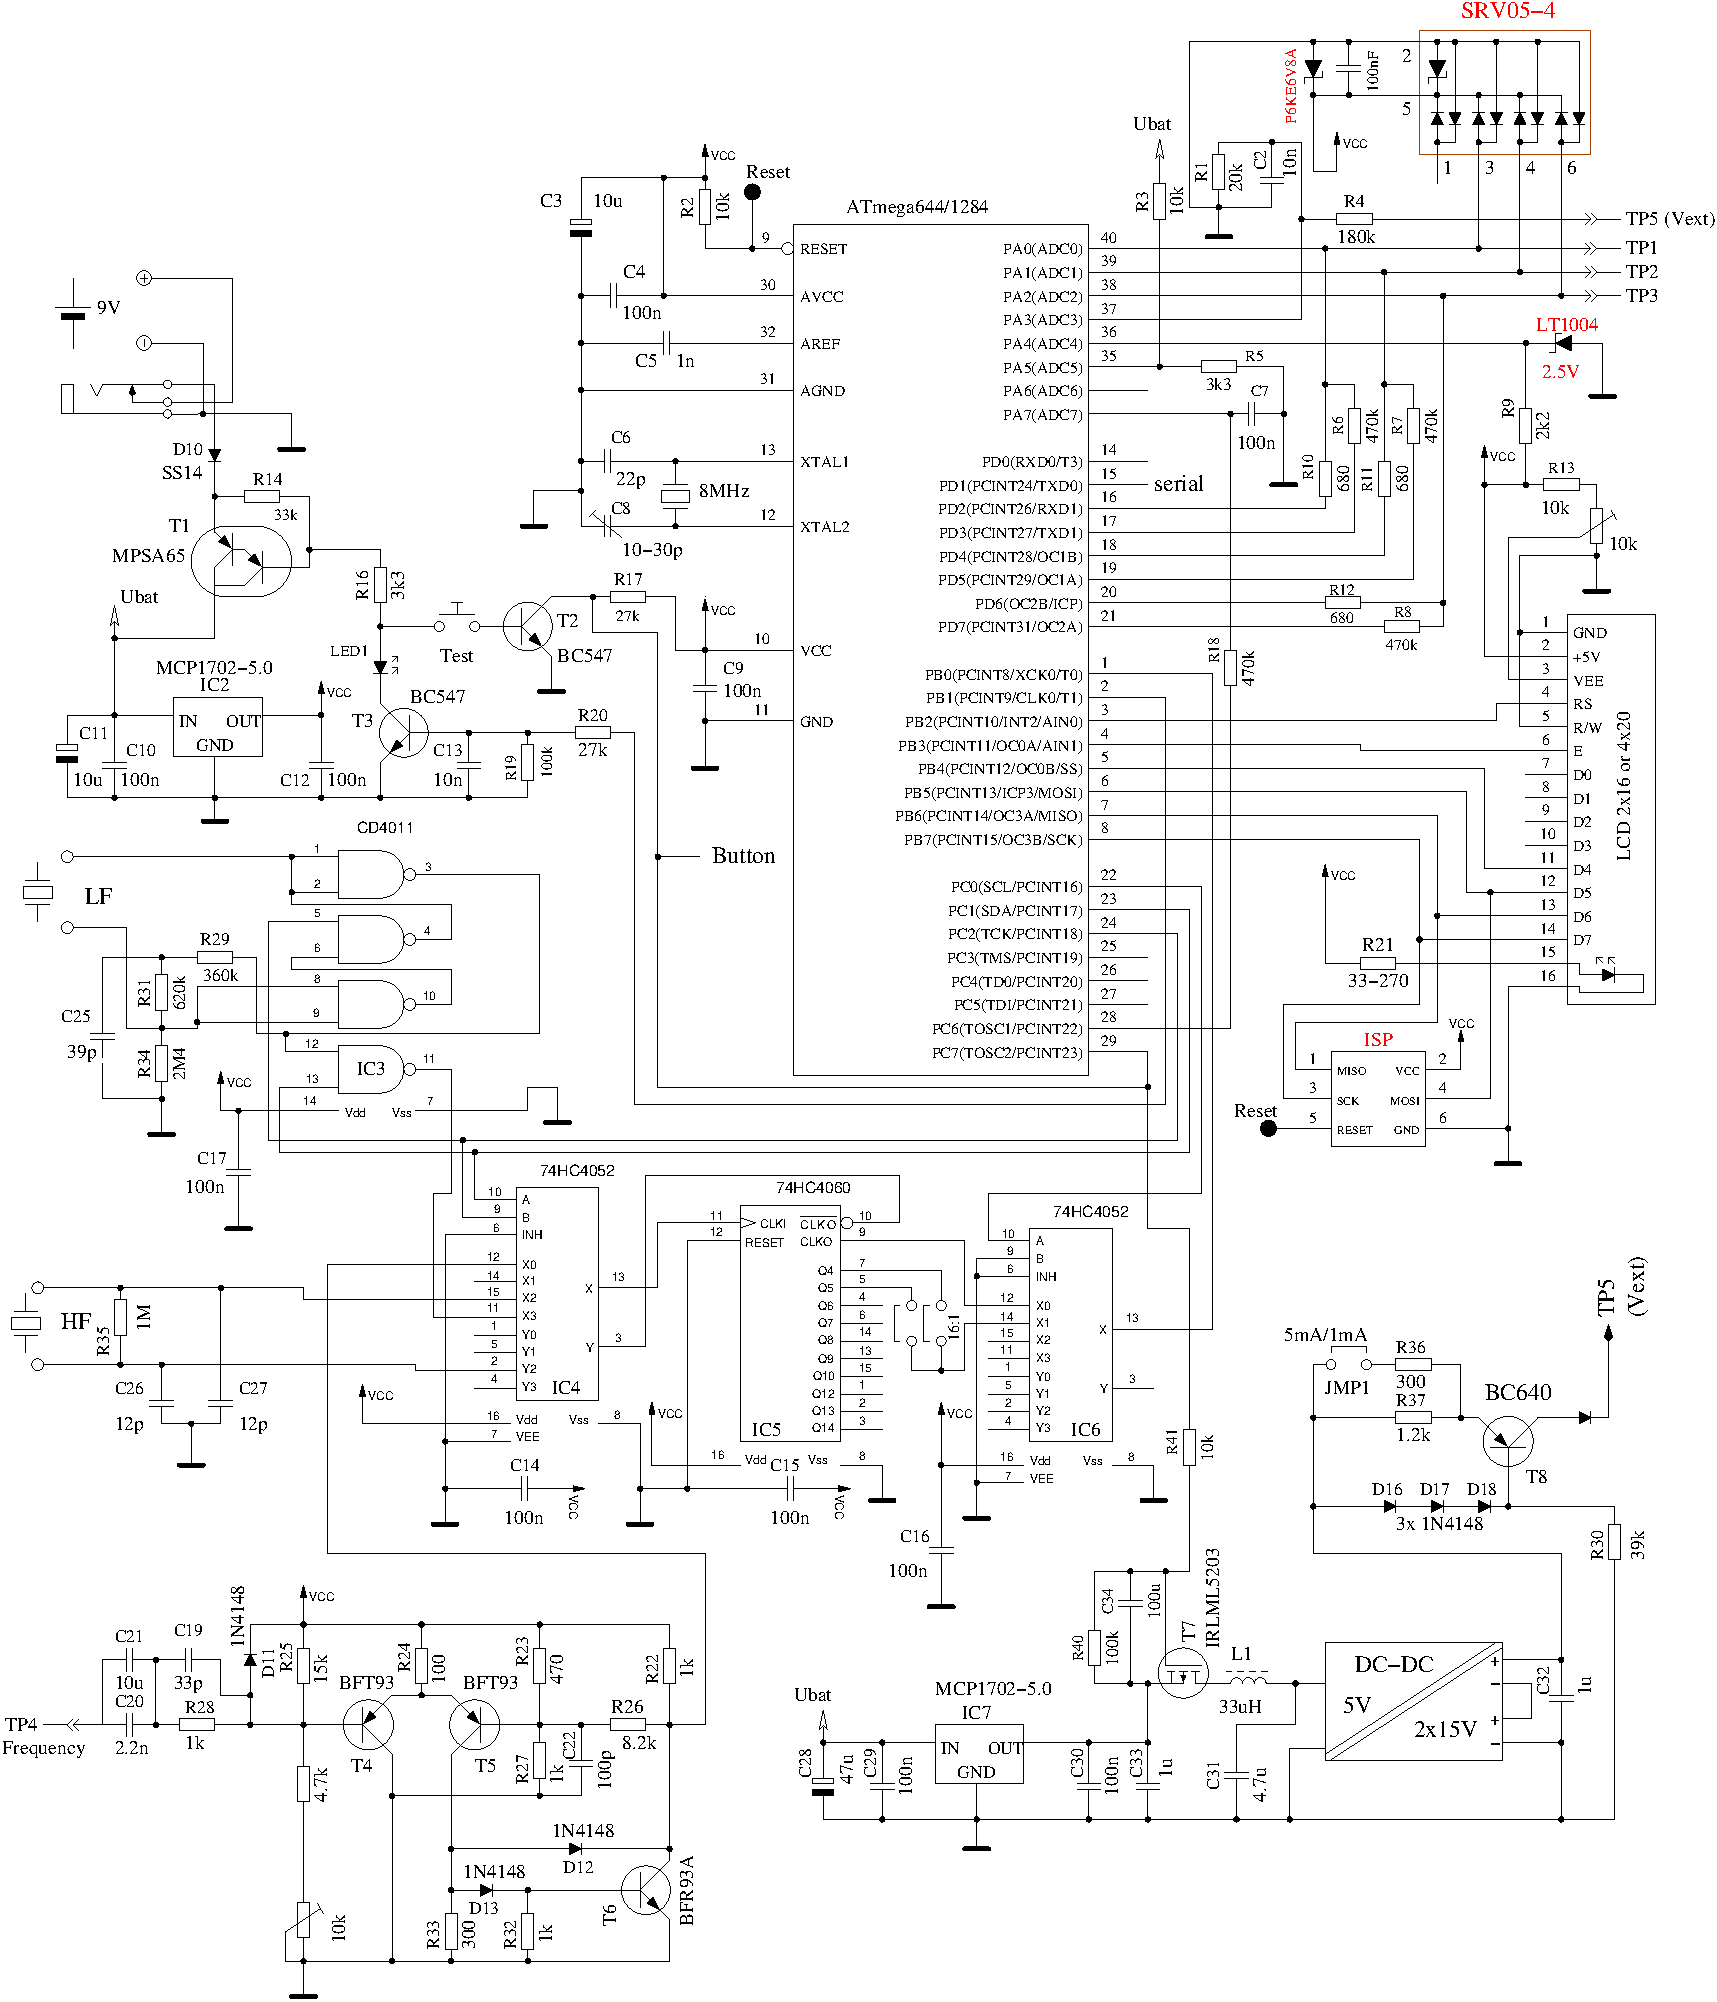
\includegraphics[width=1.\textwidth]{../FIG/t644tester.pdf}
\caption{Pokročilé schema testeru tranzistorů s ATmega644}
\label{fig:t644tester}
\end{figure}


\section{Konstrukce s ATmega1280 nebo Arduino Mega}
Základního obvodu testovacího zařízení lze také použít s Arduino Mega s ATmega1280 nebo ATmega2560
na přídavné desce.
Potřebná připojení jsou zobrazena na obrázku~\ref{fig:t1280tester}.
Zásuvná připojení přístroje Arduino pro datová připojení displeje jsou označena zelenou barvou.
Komponenty s červeným označením nejsou pro funkci testeru vyžadovány.
Mikrochip ATmega2560 má mnoho pinů, ale pouze jeden z nich má potřebné připojení pro obě metody měření frekvence. 
Tento pin musí být možné přepnout jako vstup pro počítadlo ale zároveň  musí také umět
generovat signál přerušení (interrupce) při změně úrovně.
To platí jen pro pin PE6 (T3/INT6).
Ostatní počítačové vchody jako PD7 (T0), PD6 (T1), PH7 (T4) a PL2 (T5) nelze jako interrupční signály použít.
Bohužel PE6 pin není přístupen na konektorových proužcích Arduino.
PE5 čep (7) je připojen ke kolíku 3 Arduino PWM konektor zásuvky a může být připojen
k Atmega2560 s PE6 kolíkem (8) propojený.
Výstup pro generování frekvence je na pinu PB6 (OC1B) k dispozici.
Tento pin je propojený s pinem 12 připojené PWM zásuvky.
ISP konektor není na Arduino nutný, protože lze program načíst přes USB rozhraní a zavaděč (Bootloader).
Při tom nastane jen zpoždění spuštění programu.

\begin{figure}[H]
\centering
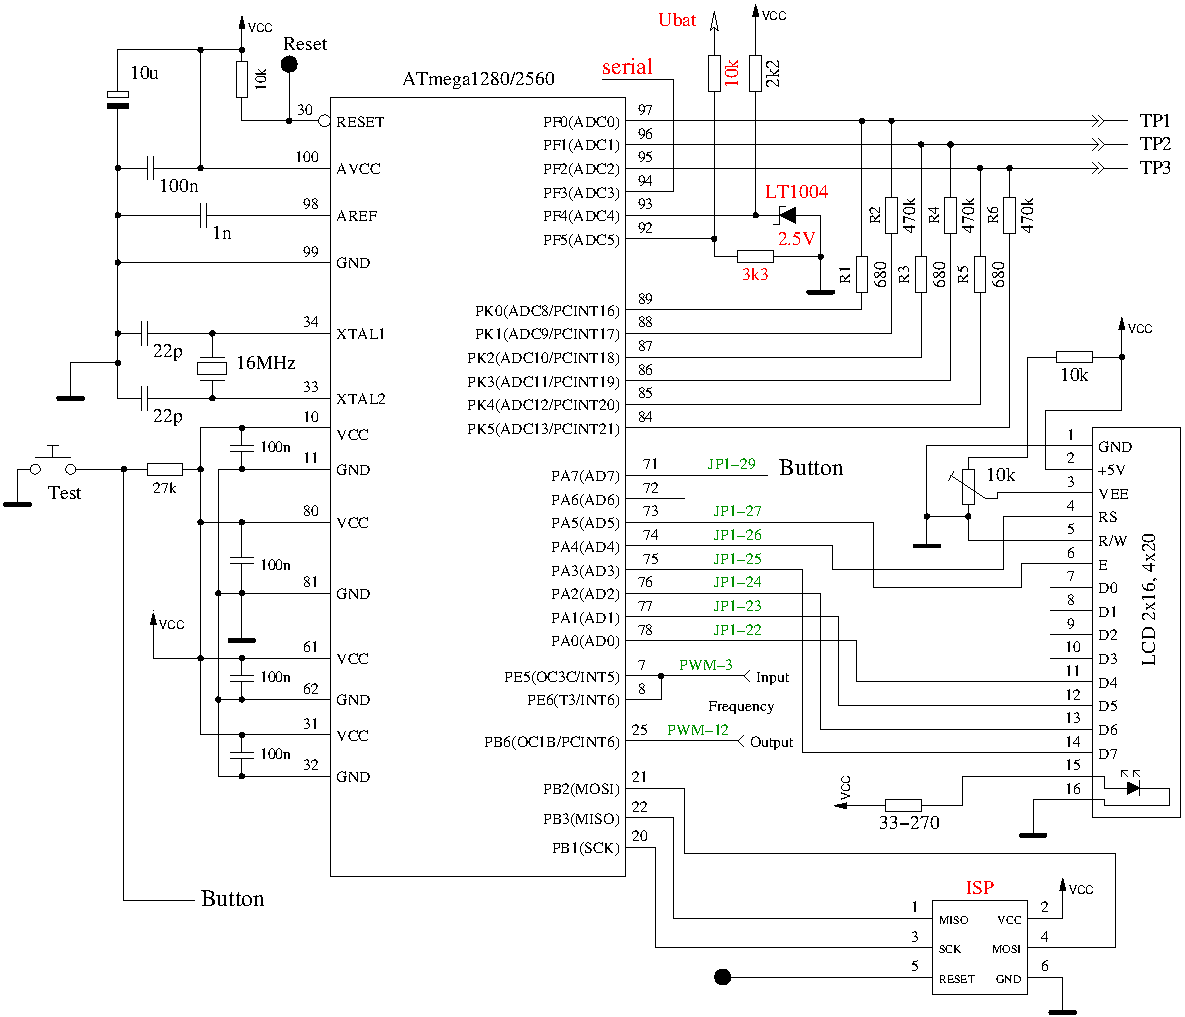
\includegraphics[width=1.\textwidth]{../FIG/t1280tester.pdf}
\caption{Tester schema s ATmega1280, ATmega2560 nebo s Arduino Mega}
\label{fig:t1280tester}
\end{figure}

Samozřejmě že všechny podporované displeje lze také připojit k ATmega1280 nebo ATmega2560, jak je uvedeno v tabulce~\ref{tab:display1280}.

\begin{table}[H]
  \begin{center}
    \begin{tabular}{| c || c | c | c | c | c | c |}
    \hline
           & Character     &  ST7565     & ST7920       & NT7108       & SSD1306     & Přídavné funkce \\
      Port & LCD           &    SPI      & seriell      & seriell      &    I\textsuperscript{2}C      & \\
    \hline
    \hline
    PA0    &  LCD-D4       &   LCD-REST  &  LCD-RESET   & HC595-RCK       &             & \\
    \hline
    PA1    &  LCD-D5       &   LCD-RS    &              & LCD-CS2        &             & kodér-2 \\
    \hline
    PA2    &  LCD-D6       &   LCD-SCLK  &              & HC164-CLK      &             & \\
    \hline
    PA3    &  LCD-D7       &   LCD-SI    &              & LCD-CS1        &             & kodér-1 \\
    \hline
    PA4    &  LCD-RS       &             &   LCD-B0     & LCD-RS         &   LCD-SDA   & \\
           &               &             &              & HC164-SER      &             & \\
    \hline
    PA5    &  LCD-E        &  (LCD-CE)   &   LCD-EN     & LCD-EN         &   LCD-SCL  & \\
    \hline
    PA7    &  Tlačítko &             &              &                &             & \\
    \hline
    \end{tabular}
  \end{center}
  \caption{Přiřazení pinů pro různé displeje na ATmega1280 / 2560}
  \label{tab:display1280}
\end{table}

\section{Čínské repliky s textovým displejem}
Tester je reprodukován v Číně podle mých znalostí ve dvou verzích s textovým displejem.
První variantou je replika prvního návrhu Markusu F. bez ISP rozhraní.
V této verzi použitý ATmega8 je  v zásuvce, takže může být také nahrazen s ATmega168 / 328.
Pro tuto verzi platí všechny pokyny v podkapitole \ref{sec:change_markus}.
Dodatečné \(100nF\) keramické kondenzátory by měly být v blízkosti ATmega VCC-GND vstupu a
pro lepší stabilitu napětí nedaleko AVCC-GND vstupu regulátoru.\\
Vzhledem k tomu, že na desce chybí ISP konektor, musí být ISP připojení dodatečně přidané nebo
procesor k programování vytažen.
Je třeba poznamenat, že i při dodatečné montáži krystalu musí ISP-Programátor dostat externí takt,
nebo musí být programovací základna vybavena krystalem.
Druhá varianta je z velké části postavena v SMD technologii. Také použitý ATmega168 nebo ATmega328
je typu 32TQFP a pevně naletován.
Pro programování na desce je k dispozici 10 pólový ISP konektor.
Já  jsem analyzoval verzi ,,2.1 2012/11/06'' .Zde je chyba v součástce ,,D1'',
což mělo být referenční \(2,5V\) napětí. Ve skutečnosti je vybaven Zenerovou diodou.
Tato součástka by měla být odstraněna. Použít jze přesnou referenci jako LM4040AIZ2.5 nebo
LT1004CZ-2.5. Chybějící přesná reference je softwarem ale detekována, tak že ta výměna
není tak podstatná.
V mém exempláři byla instalovaná softwarová verse 1.02k. 10-pólová ISP-zástrčka nebyla obsazena
a já jsem  musel dodatečně spojit pin 6 a 10. Můj programátor očekává GND na pinu 10, ale
testovaném přístroji měl konektor GND pouze na pinech 4 a 6.
ATmega168 označení bylo vyškrábané a dokumentace nebyla k dispozici.
Bezpečnostní bity ATmega byly tak nastaveny, aby nebylo možné program číst.
Mohl jsem ale snadno nainstalovat softwarovou verzi 1.05k.
Tato softwarová verze dělala problémy u jiného exempláře s výrobní verzí "2.2 2012/11/26".
Zde běžela až poté, když jsem přidal další SMD \(100nF\) kondenzátor mezi piny 18-AVCC
a 21-GND. Software 1.05k využívá při čekání stav spánku ATmega.
Proto se spotřeba energie častěji mění a regulátor napětí je více namáhaný.
Dále jsem si všiml,že pro zlepšení stability VCC napětí, je kromě \(100nF\) keramického kondenzátoru
ještě jeden \(220\mu F\) elektrolytický kondenzátor použitý v blízkosti 78L05-regulátoru napětí.
Napájecí \(9V\) napětí je vybaveno stejnými kondenzátory, až na to, že jsou na emitoru PNP-Transistoru
(paralelně k baterii), místo přímo u řadiče napětí.
Vodiče tištěných spojů mezi ATmega a testovacími porty jsou částečně velmi tenké. Já měřil asi \(100m\Omega\)
pro jednu signální cestu. To je důvod, proč při s \(0\Omega\) spojenými piny, naměříte \(0,3\Omega\) .
Při měření v ESR režimu je toto možné obvykle kompenzovat nulováním.
Od softwarové verse 1.07K jsou při měření odporů pod \(10\Omega\) automaticky offsety, zjištěny při
auto-diagnose vzaty v úvahu.

\section{Čínské repliky s grafickým displejem}
Novější repliky používají grafický displej s rozsahem 128x64 pixelů, například verze Fish8840.
Tato verze používá modifikovaný okruh pro zapnutí. Obrázek \ref{fig:Fish8840} ukazuje část obvodu.

\begin{figure}[H]
\centering
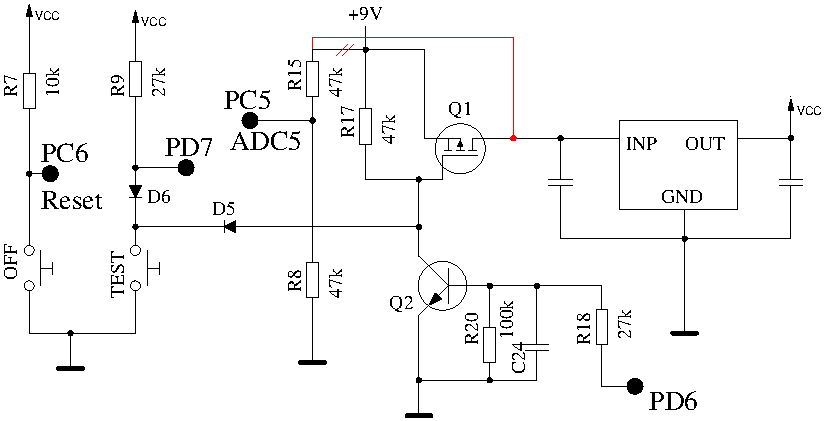
\includegraphics[width=.7\textwidth]{../FIG/Fish8840.pdf}
\caption{Výňatek z obvodu Fish8840}
\label{fig:Fish8840}
\end{figure}

Jak je z odporů R8 a R15 zřejmé, je zde při poměru 2: 1 odlišný poměr dělitelů napětí akumulátoru
než v původním provedení.
Kromě toho je R15 připojen přímo k baterii, což vede k nízké spotřebě energie v baterii
i ve vypnutém stavu. Zde by měl být R15 lépe připojen na dra-in od Q1 nebo na vstup regulátoru napětí, aby
se zabránilo zbytečné spotřebě baterie.
Odpovídající změny ukazuje obrázek \ref{fig:Fish8840patch}. Tištěný spoj je mezi  R17 a D5 přerušen
a pomocí smaltovaného měděného drátu nové spojení mezi Q1 a R15 uděláno.

\begin{figure}[H]
\centering
\includegraphics[width=.7\textwidth]{../PNG/Fish8840patch.jpg}
\caption{Fotografie upravené desky Fish8840}
\label{fig:Fish8840patch}
\end{figure}

Poměr děliče napětí musí být v každém případě v konfiguraci v souboru Makefile specifikován 
před načtením softwaru (například s BAT\_NUMERATOR=66).
Displej Modul Fish8840 testeru má \(3.3V\) regulátor napětí, který řídí provozní napětí kontroléru
displeje.
Protože datové linky modulu displeje přicházejí z \(5V\) ATmega výstupů, je zde to \(3.3V\) napětí
zvýšené.
Odpomoc nabízí malý adaptér, podle obrázku \ref{fig:Fish8840Adapt}. Na něm jsou čtyři \(2.7k\Omega\)
odpory zapojeny v řadě k datovým linkám.
K připojení displeje s adaptérem k Fish8840 testeru je nezbytné prodloužení závitovými distančními sloupky M3.

\begin{figure}[H]
  \begin{subfigure}[b]{.5\textwidth}
    \centering
    \includegraphics[width=1.\textwidth]{../PNG/Fish8840Adapt1.jpg}
    \caption{Displej s adaptérem}
  \end{subfigure}
  ~
  \begin{subfigure}[b]{.5\textwidth}
    \centering
    \includegraphics[width=1.\textwidth]{../PNG/Fish8840Adapt2.jpg}
    \caption{Smontovaný Tester}
  \end{subfigure}
  \caption{Adaptér se správné zapojeným displejem}
  \label{fig:Fish8840Adapt}
\end{figure}

Namísto této úpravy je nyní možné v Makefile volbou LCD\_SPI\_OPEN\_COL použít také se speciálním nastavením
ATmega výstupů při použíti 4-SPI signálů.
V tomto případě nejsou výstupy připojeny k VCC, ale při vydání vysoké úrovně, pouze přes
interní ,,Pull-Up'' odpory.
Je-li nastavena volba PULLUP\_DISABLE, je pro resetovací signál (PD0) externí ,,Pull-Up'' odpor vyžadován.
Vzhledem k tomu, datové signály nejsou nyní nikdy přepnuty přímo k VCC, nebude to  \(3.3V\)
napětí řídící jednotky LCD zvýšeno.
Můj exemplář Fish8840 Testeru má všechny signály pro připojení textového displeje k disposici. 
Proto může být také vybavený textovým displejem, pokud je přípoj doplněn o potenciometr pro nastavení kontrastu.
Napájecí pin 15 pro osvětlení pozadí je ale přímo připojen na VCC.
V případě instalace textového displeje, je třeba dbát na sériový odpor pro LED.
Samozřejmě, musí být softwarová verse na jiný displej přizpůsobena.
Fish8840 deska DPS nabízí také možnosti softwarové modifikace.
Pro funkční schopnost nemůže být, samozřejmě, žádná záruka poskytnuta.
Protože jsou bezpečnostní bity v ATmega328 jedno-čipu nastaveny, není možné,
stav původní čínské softwarové verse zálohovat.

Tím pádem... bohužel... nevede, zpět k původní verzi softwaru, žádná cesta.


Další verzí s grafickým displejem je model WEI\_M8 , který je znázorněn na obrázku \ref{fig:WeiM8}.
Tato replika používá, jako zdroj energie, Li Ion akumulátor typu AA (Mig-non), který lze přes
mi-kro-USB rozhraní nabít. Provoz je i bez baterie přes USB rozhraní možný.

\begin{figure}[H]
\centering
\includegraphics[width=.7\textwidth]{../PNG/WEI_M8.JPG}
\caption{Fotografie čínského WEI\_M8 Testeru}
\label{fig:WeiM8}
\end{figure}

Je příjemné, že na desce adaptéru displeje, jsou již sériové odpory pro signální linky, jak je vidět
na levém obrázku ~\ref{fig:WeiM8int}. Tím nehrozí zvýšení dodávky \(3.3V\) napětí pro řadič displeje kvůli
ATmega \(5V\) úrovni napětí výstupního signálu.

\begin{figure}[H]
  \begin{subfigure}[b]{.5\textwidth}
    \centering
    \includegraphics[width=1.\textwidth]{../PNG/WEI_M8_D.JPG}
    \caption{Deska adaptéru pro displej}
  \end{subfigure}
  ~
  \begin{subfigure}[b]{.5\textwidth}
    \centering
    \includegraphics[width=1.\textwidth]{../PNG/WEI_M8_L.JPG}
    \caption{Základní deska}
  \end{subfigure}
  \caption{Pohled na  WEI\_M8 tester}
  \label{fig:WeiM8int}
\end{figure}


Při upgradu softwaru na versi 1.12k jsem se setkal s některými obtížemi.
Pokud je ATmega pojistka nastavena podle doporučení na 0x04 (nebo 0xfc), došlo při určitých měření
k ,,brown out'' resetu procesoru.
Příčinou tohoto chování jsou krátkodobé poklesy napětí VCC napájení.
Přidal jsem proto  \(4.7\mu F\) keramický kondenzátor na vstup regulátoru napětí
a další \(10\mu F\) keramický kondenzátor na vstup (VCC) zdroje.
Jak před, tak i po té modifikaci byl u bipolárních transistorů měřen zbytkový proud kolektoru (ICEO nebo ICEs).
Teprve výměna toho LDO-regulátoru napětí (neznámého typu) za MCP1702-5002 pomohla.
Na obrázku \ref{fig:WeiM8mod} je vidět vložený akumulátor,
modifikace desky DPS s MCP1702 regulátorem a napravo pod ním šikmo naletované kondenzátory.
Pokud nechcete aktualizovat kondenzátory, nastavte ATmexa pojistku na 0x07 (0xff).
S tímto nastavením je provoz možný.
Poklesy napětí nebudou ale hlídané.

\begin{figure}[H]
\centering
\includegraphics[width=.7\textwidth]{../PNG/WEI_M8_modified.JPG}
\caption{Fotografie modifikovaného WEI\_M8 testeru}
\label{fig:WeiM8mod}
\end{figure}

Další verzí s grafickým LCD displejem je T4 Tester na žluté desce.
Při přehrávání nového softwaru jsem musel odstranit displej.
Na pravé fotografii obrázku \ref{fig:T4_front} je, v pravém horním rohu,
 položen konektor pro ISP připojení
vedle odpovídajících otvorů na desce ve správné orientaci.
Pro programování jsem zástrčku nenaletoval, ale pouze nastrčil a pevným bočním tlakem prstu po dobu
programování zajistil.
To umožňuje snadno vyjmout konektoru po programování a vrácení displeje na původní místo.
Mimochodem, software 1.12k lze snadno načíst.
Také aktivace ,,Brown-Out'' detekce procesoru s ATmega pojistkou nepřinesla žádné překvapení.

\begin{figure}[H]
  \begin{subfigure}[b]{.5\textwidth}
    \centering
    \includegraphics[width=1.\textwidth]{../PNG/T4_front.JPG}
    \caption{Kompletní}
  \end{subfigure}
  ~
  \begin{subfigure}[b]{.5\textwidth}
    \centering
    \includegraphics[width=1.\textwidth]{../PNG/T4_front_noLCD.JPG}
    \caption{S odebraným displejem}
  \end{subfigure}
  \caption{Pohled zepředu na T4 tester}
  \label{fig:T4_front}
\end{figure}

Na fotografiích zadní strany na obrázku \ref{fig:T4_back} vidíte dodatečné dodané
závitové \(5mm\) šrouby a napájené kabely s měřícími svorkami.
Protože pro datové signály grafického LCD kontroléru žádné nastavení
signálu (\(5V~-\textgreater ~3.3V\)) neexistuje, doporučuji volbu LCD\_SPI\_OPEN\_COL.
Protože zde dodatečně instalace ,,pull-up'' odporu k "vytažení" signálu SPI reset
není lehce proveditelná, zůstává jen volba DISABLE\_PULLUP . 
Pro následné expanze je tato verze testeru méně vhodná, protože i výměna displeje je zde obtížná.

\begin{figure}[H]
  \begin{subfigure}[b]{.5\textwidth}
    \centering
    \includegraphics[width=1.\textwidth]{../PNG/T4_back.JPG}
    \caption{Přední strana}
  \end{subfigure}
  ~
  \begin{subfigure}[b]{.5\textwidth}
    \centering
    \includegraphics[width=1.\textwidth]{../PNG/T4_back_clips.JPG}
    \caption{S měřícími kabely}
  \end{subfigure}
  \caption{Pohled zezadu na T4}
  \label{fig:T4_back}
\end{figure}

Další čínská verze s grafickým displejem je nabízena s označením "GM328".
V této verzi je grafický displej umístěn přes 16 kolíkovou zásuvku na přídavné desce. Na ní je také
PD5 přes pin 6 CE (chip enable) signál grafické řídicí jednotky připojen. Tento signál je zde ale
také s \(0V\) Power (GND) spojený. 
To způsobí zkrat, při pokusu tento ATmega pin přepnout jako \(5V\) výstup.
Novější verze softwaru také přepínají CE signál, i když není k provozu potřebný.
Proto je nutné, před nahráním nové softwarové verze, na přídavné desce DPS kontakt 6 u zásuvky
přerušit.

\section{Čínské soupravy a rotačním kodérem}

Dosud jsou známy dva sady s grafickým displejem a rotačním enkodérem.
První klon používá displej s ST7565 nebo kompatibilním řadičem (128x64 pixelů).
Kromě otočného enkodéru je k dispozici vstup pro měření frekvence.
Pro testovací porty je 14 kolíková zásuvka Textool, 3 pájecí očka pro drát,
stejně jako zkušební podložka pro SMD komponenty k dispozici. 
Fotografie~\ref{fig:Kit_mono} zobrazují smontovanou sestavu. Jeden ze dvou \(22 pF\) kondenzátorů 
byl nahrazen trimrem což umožňuje přesnější nastavení frekvence křemene při měření
frekvence nebo její generování.
\begin{figure}[H]
  \begin{subfigure}[b]{.5\textwidth}
    \centering
    \includegraphics[width=1.\textwidth]{../PNG/Kit_ST7565a.jpg}
    \caption{Smontován}
  \end{subfigure}
  ~
  \begin{subfigure}[b]{.5\textwidth}
    \centering
    \includegraphics[width=1.\textwidth]{../PNG/Kit_ST7565b.jpg}
    \caption{s odebraným displejem}
  \end{subfigure}
  \caption{Sestavená sada s 128x64 pixelovým displejem}
  \label{fig:Kit_mono}
\end{figure}

Později zveřejněná sada využívá barevného displeje s ST7735 řadičem (128x160 pixelů) a má kromě
vstupního signálu pro měření napětí a frekvence ještě frekvenční výstup.
Frekvenční výstup není vyrovnán, ale je pouze paralelně připojen k TP2.
Při měření napětí je pouze možné měřit pozitivní stejnosměrné napětí až 50V DC-DC.
Převodník pro měření zenerova napětí nebyl plánován.
Fotografie \ref{fig:Kit_color} zobrazují smontované sestavy.
I zde byl jeden ze dvou \(22 pF\) kondenzátorů byl nahrazen trimrem (zelený). 

\begin{figure}[H]
  \begin{subfigure}[b]{.5\textwidth}
    \centering
    \includegraphics[width=1.\textwidth]{../PNG/Kit_Color_a.jpg}
    \caption{Sestaven}
  \end{subfigure}
  ~
  \begin{subfigure}[b]{.5\textwidth}
    \centering
    \includegraphics[width=1.\textwidth]{../PNG/Kit_Color_b.jpg}
    \caption{Odebraný displej}
  \end{subfigure}
  \caption{Sestavená sada s 160x128 pixelovým displejem}
  \label{fig:Kit_color}
\end{figure}

Obě sady používají ATmega328P verzi s PATICI DIP a nemají žádný ISP konektor pro instalaci nových
verzí softwaru.
První verze používá pro základní desku DSP pouze součástky s drátovými vývody.
Měřicí odpory \(680\Omega\) a \(470k\Omega\) byly v mé sadě s 0.1\% tolerancí dodány.
Dokonce i \(220 nF\) kondenzátor pro kalibraci v soupravě nescházel.
Souprava s barevným displejem má kromě připojení 9V baterie zásuvku pro napájení.
SMD komponenty byly již na desce obsazeny, takže i při této sadě je třeba provádět pouze jednoduché pájení.
Malou nevýhodou verze s barevným displejem je rychlost výstupu.
Zejména při provozu v menu je výrazně pomalejší výstup negativní.
Na druhé straně má barevný displej výrazně vyšší počet pixelů a může tak představovat více textu.
Obě sady používají regulátor napětí pro napájení 3,3V na plně obsazeném displeji.
Pouze kontakty konektoru musí být na desce displeje naletovány.
Barevná verze používá vyrovnávací paměť CD4050 pro nastavení úrovní signálu.
Na zobrazovací desce varianta ST7565 není vidět žádné nastavení úrovně signálu.
Pravděpodobně vybraná verze regulátoru toleruje úrovně signálu 5V ATmega328.
V žádném případě není žádná ochranná dioda proti napájení 3,3 V v tomto regulátoru viditelná.

\section{Ještě tester od firmy Hiland s M644}
Tento  klone je postaven podle plánu \ref{fig:t644tester} na straně \pageref{T644}. od Nika Lanchaka s Ukrajiny.
Tester je ovládán \textbf {tlačítkem}, které je zároveň \textbf {rotační} snímač.
\vspace{0,5cm}
Nabízí následující přídavky:
\vspace{-1.5\baselineskip}
\begin{itemize} \setlength{\itemsep}{-0.5\baselineskip}
 \item měření a generaci frekvence
 \item den f-Generator
 \item 10-bitový PWM,
 \item Impulsdrehgeber
 \item měření krystalů
 \item měření napětí a Zenerových diod(až do 50V).
\end{itemize}
\vspace{-0.5\baselineskip}
Na desce je pod displejem připravena 6ti pólová řada pro ISP rozhraní s následujícím zapojením:\\
\textbf {z leva do prava}: 1~-Reset; 2~-SCK; 3~-MISO; 4~-MOSI; 5~-+5V; 6~-GND.\\
Aby bylo možné tester aktualizovat je třeba mít modifikovaný kabel, který lze relativně lehce vyrobit.
Při dodání jsou na desce dvě řady zdířek a testovací sokl je volně přiložen.

U toho níže zobrazeného testeru, byl sokl přímo naletován a tím ušetřená zdířková řada naletována na přestřižený vlastní kabel a zajištěna smršťovací bužírkou.  
\begin{figure}[H]
 \centering
 \begin{overpic}[width=.64\textwidth]{../FIG/Kabel_Hiland.pdf}
  \color{black}
  \put(14,99){\makebox(0,0)[cb]{Programátor}}
  \put(14,-3){\makebox(0,0)[cb]{konektor}}
  \put(49,99){\makebox(0,0)[cb]{Pohled shora}}
  \put(38,-3){\makebox(0,0)[lb]{Plochý kabel}}
  \put(90,99){\makebox(0,0)[cb]{tester}}
  \put(90,-3){\makebox(0,0)[cb]{zdířková řada}}
 \end{overpic}
 \caption{6 a 10 ti pólové upravené kabely k programování}
\end{figure}
\begin{figure}[H]
  \begin{subfigure}[b]{.5\textwidth}
    \centering
    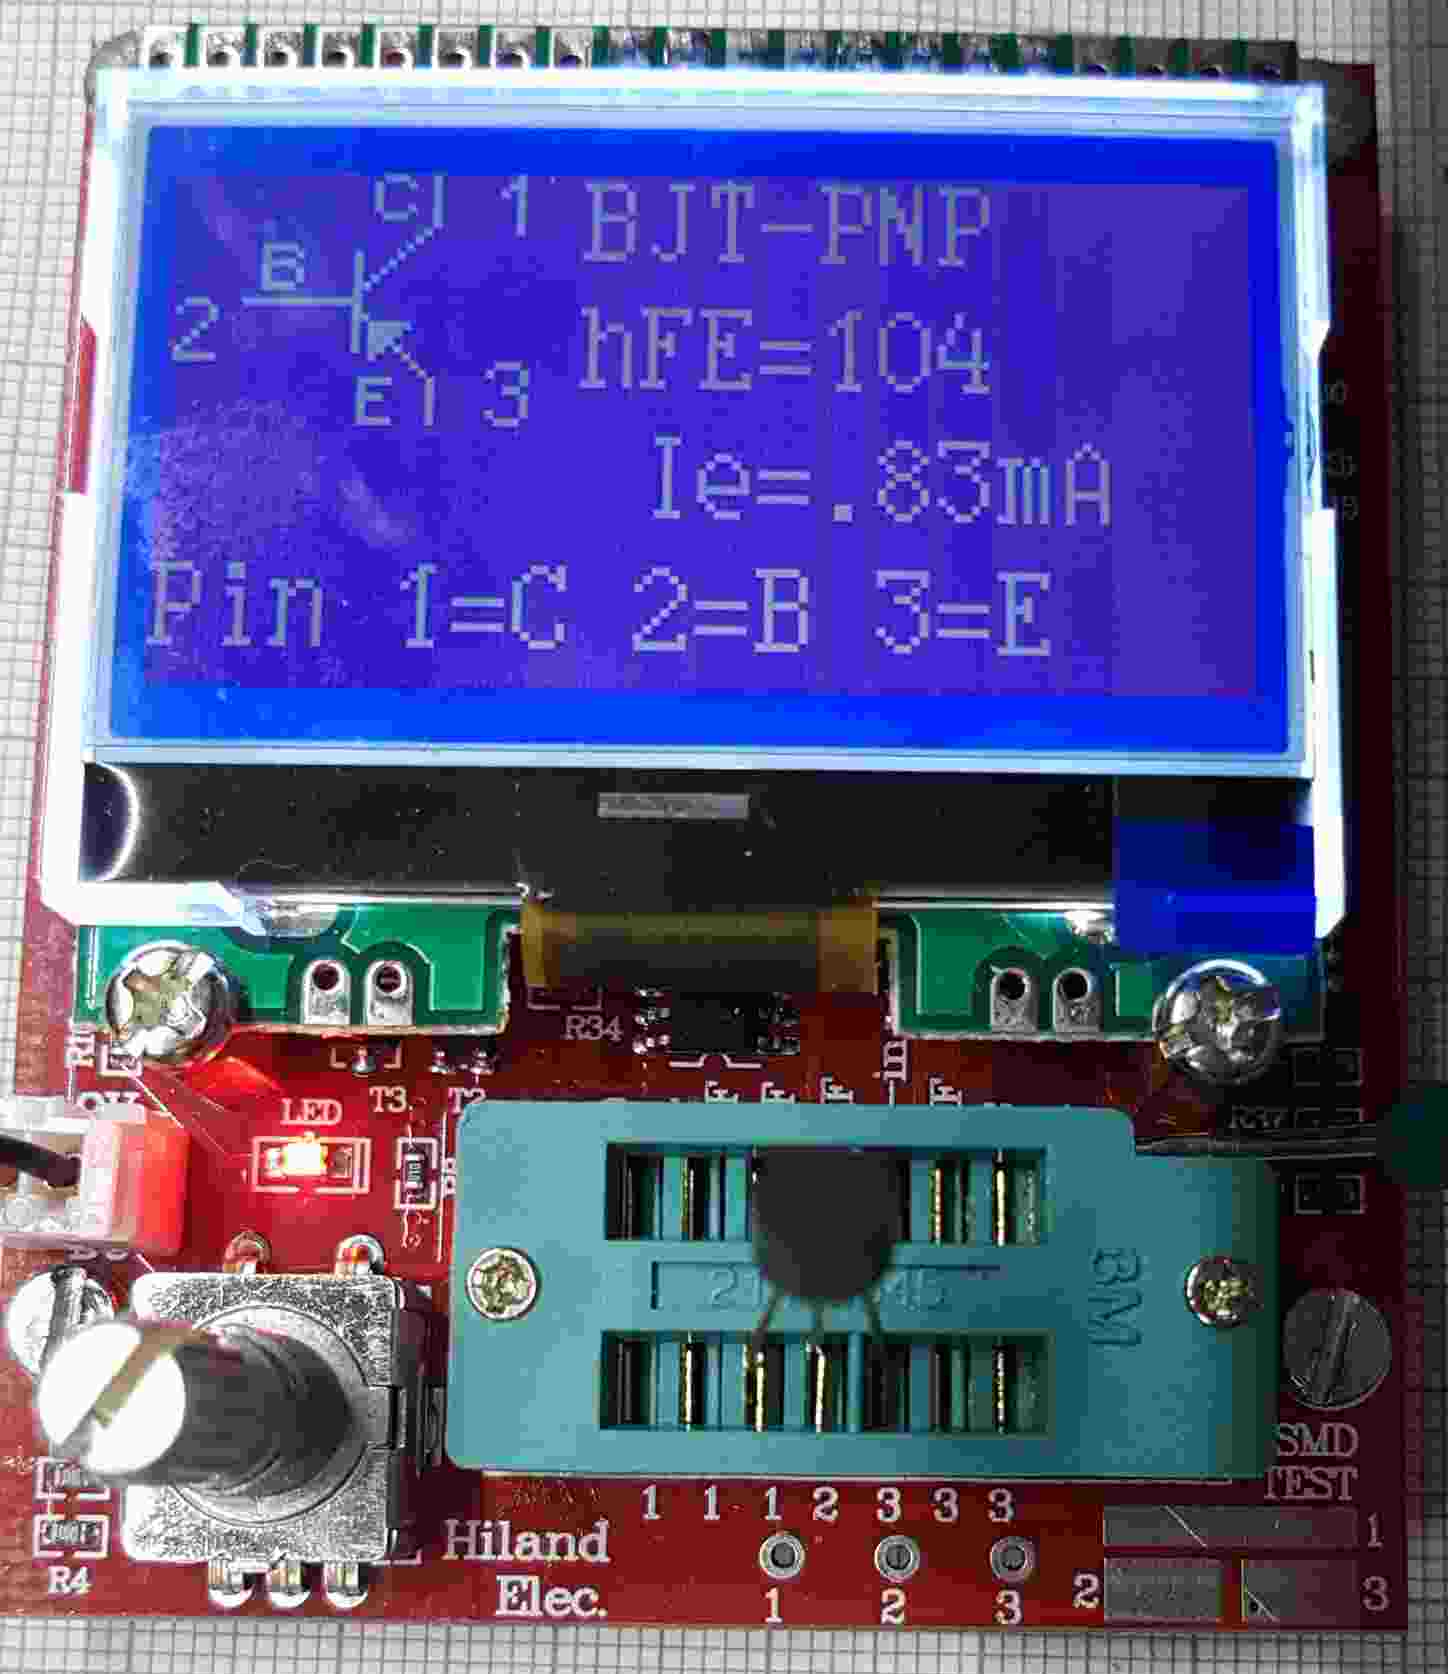
\includegraphics[width=.875\textwidth]{../PNG/Hi_u.jpg}
    \caption{dole TP1 až TP3 pro identifikaci součástek}
  \end{subfigure}
  ~
  \begin{subfigure}[b]{.5\textwidth}
    \centering
    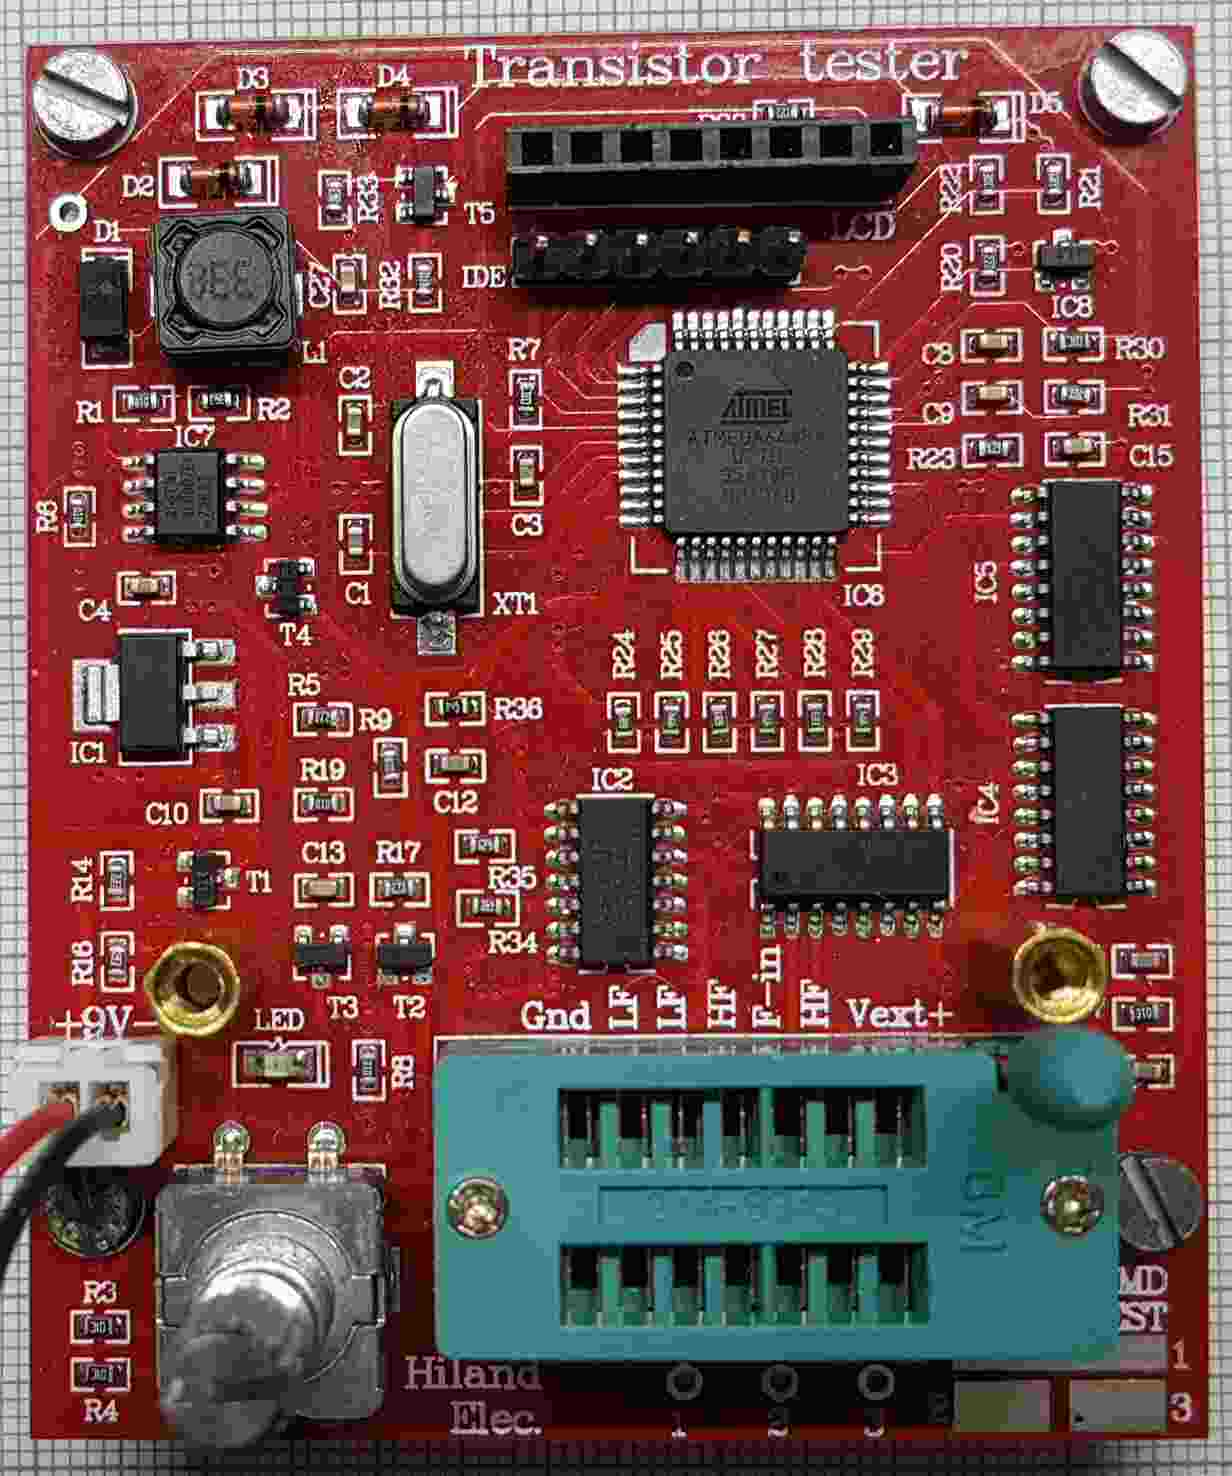
\includegraphics[width=.756\textwidth]{../PNG/Hi_o.jpg}
    \caption{nahoře TP pro funkce menu a IDE}
  \end{subfigure}
  \caption{Tester firmy Hiland s testovacím soklem a 128x64 Pixel LCD Displejem}
  \label{fig:Hiland}
\end{figure}

{\textbf {Die Testovací piny TP1, TP2 und TP3}} lsou určeny pro automatické zjištění a měření součástek a jsou popsány čísly {\textbf {1~~1~~1~~2~~3~~3~~3}}.

Stejná čísla jsou také SMD poli a kromě toho je možné, naletovat vlastní kabely.

Der \textbf {Testovací pin TP2} má kromě toho funkci výstupu v menu ,,f-Generator''.
\\S \textbf{ LF} označené piny jsou určeny k měření krystalu s nízkou rezonanční frekvencí,
\\a \textbf{ HF} označené piny, jsou pro měření krystalu s vysokou rezonanční frekvencí.
\\
Pin \textbf {F-in} lze použít dohromady {\textbf {Gnd}} pro menu funkci měření frekvence.
\\a \textbf {Vext+} právě tak s {\textbf {Gnd}} k měření napětí {\textbf a} k určení Zenerových diod.\\

Poznámka překladatele. Nově existuje k tomuto testeru návod v češtině.

